\chapter{绪论}
\section{研究背景与意义}
\subsection{人口老龄化加剧下的移动通信终端使用困境}
伴随我国人口结构的深刻变化，老龄化已成为关乎国计民生的重要社会议题。根据国家统计局发布的数据，截至2023年末，我国60岁及以上人口已达2.97亿，占总人口的21.1\,\%\upcite{1}，预计到2035年这一比例将突破30\%，我国正稳步迈向中度老龄化社会。在通信技术高速发展的背景下，移动通信终端早已超越传统的语音通话功能，演变为集即时通讯、移动支付、远程医疗、出行导航等多重服务于一体的综合数字生活入口，深度融入了现代社会的各个角落。


\begin{figure}[htbp]
    \centering
    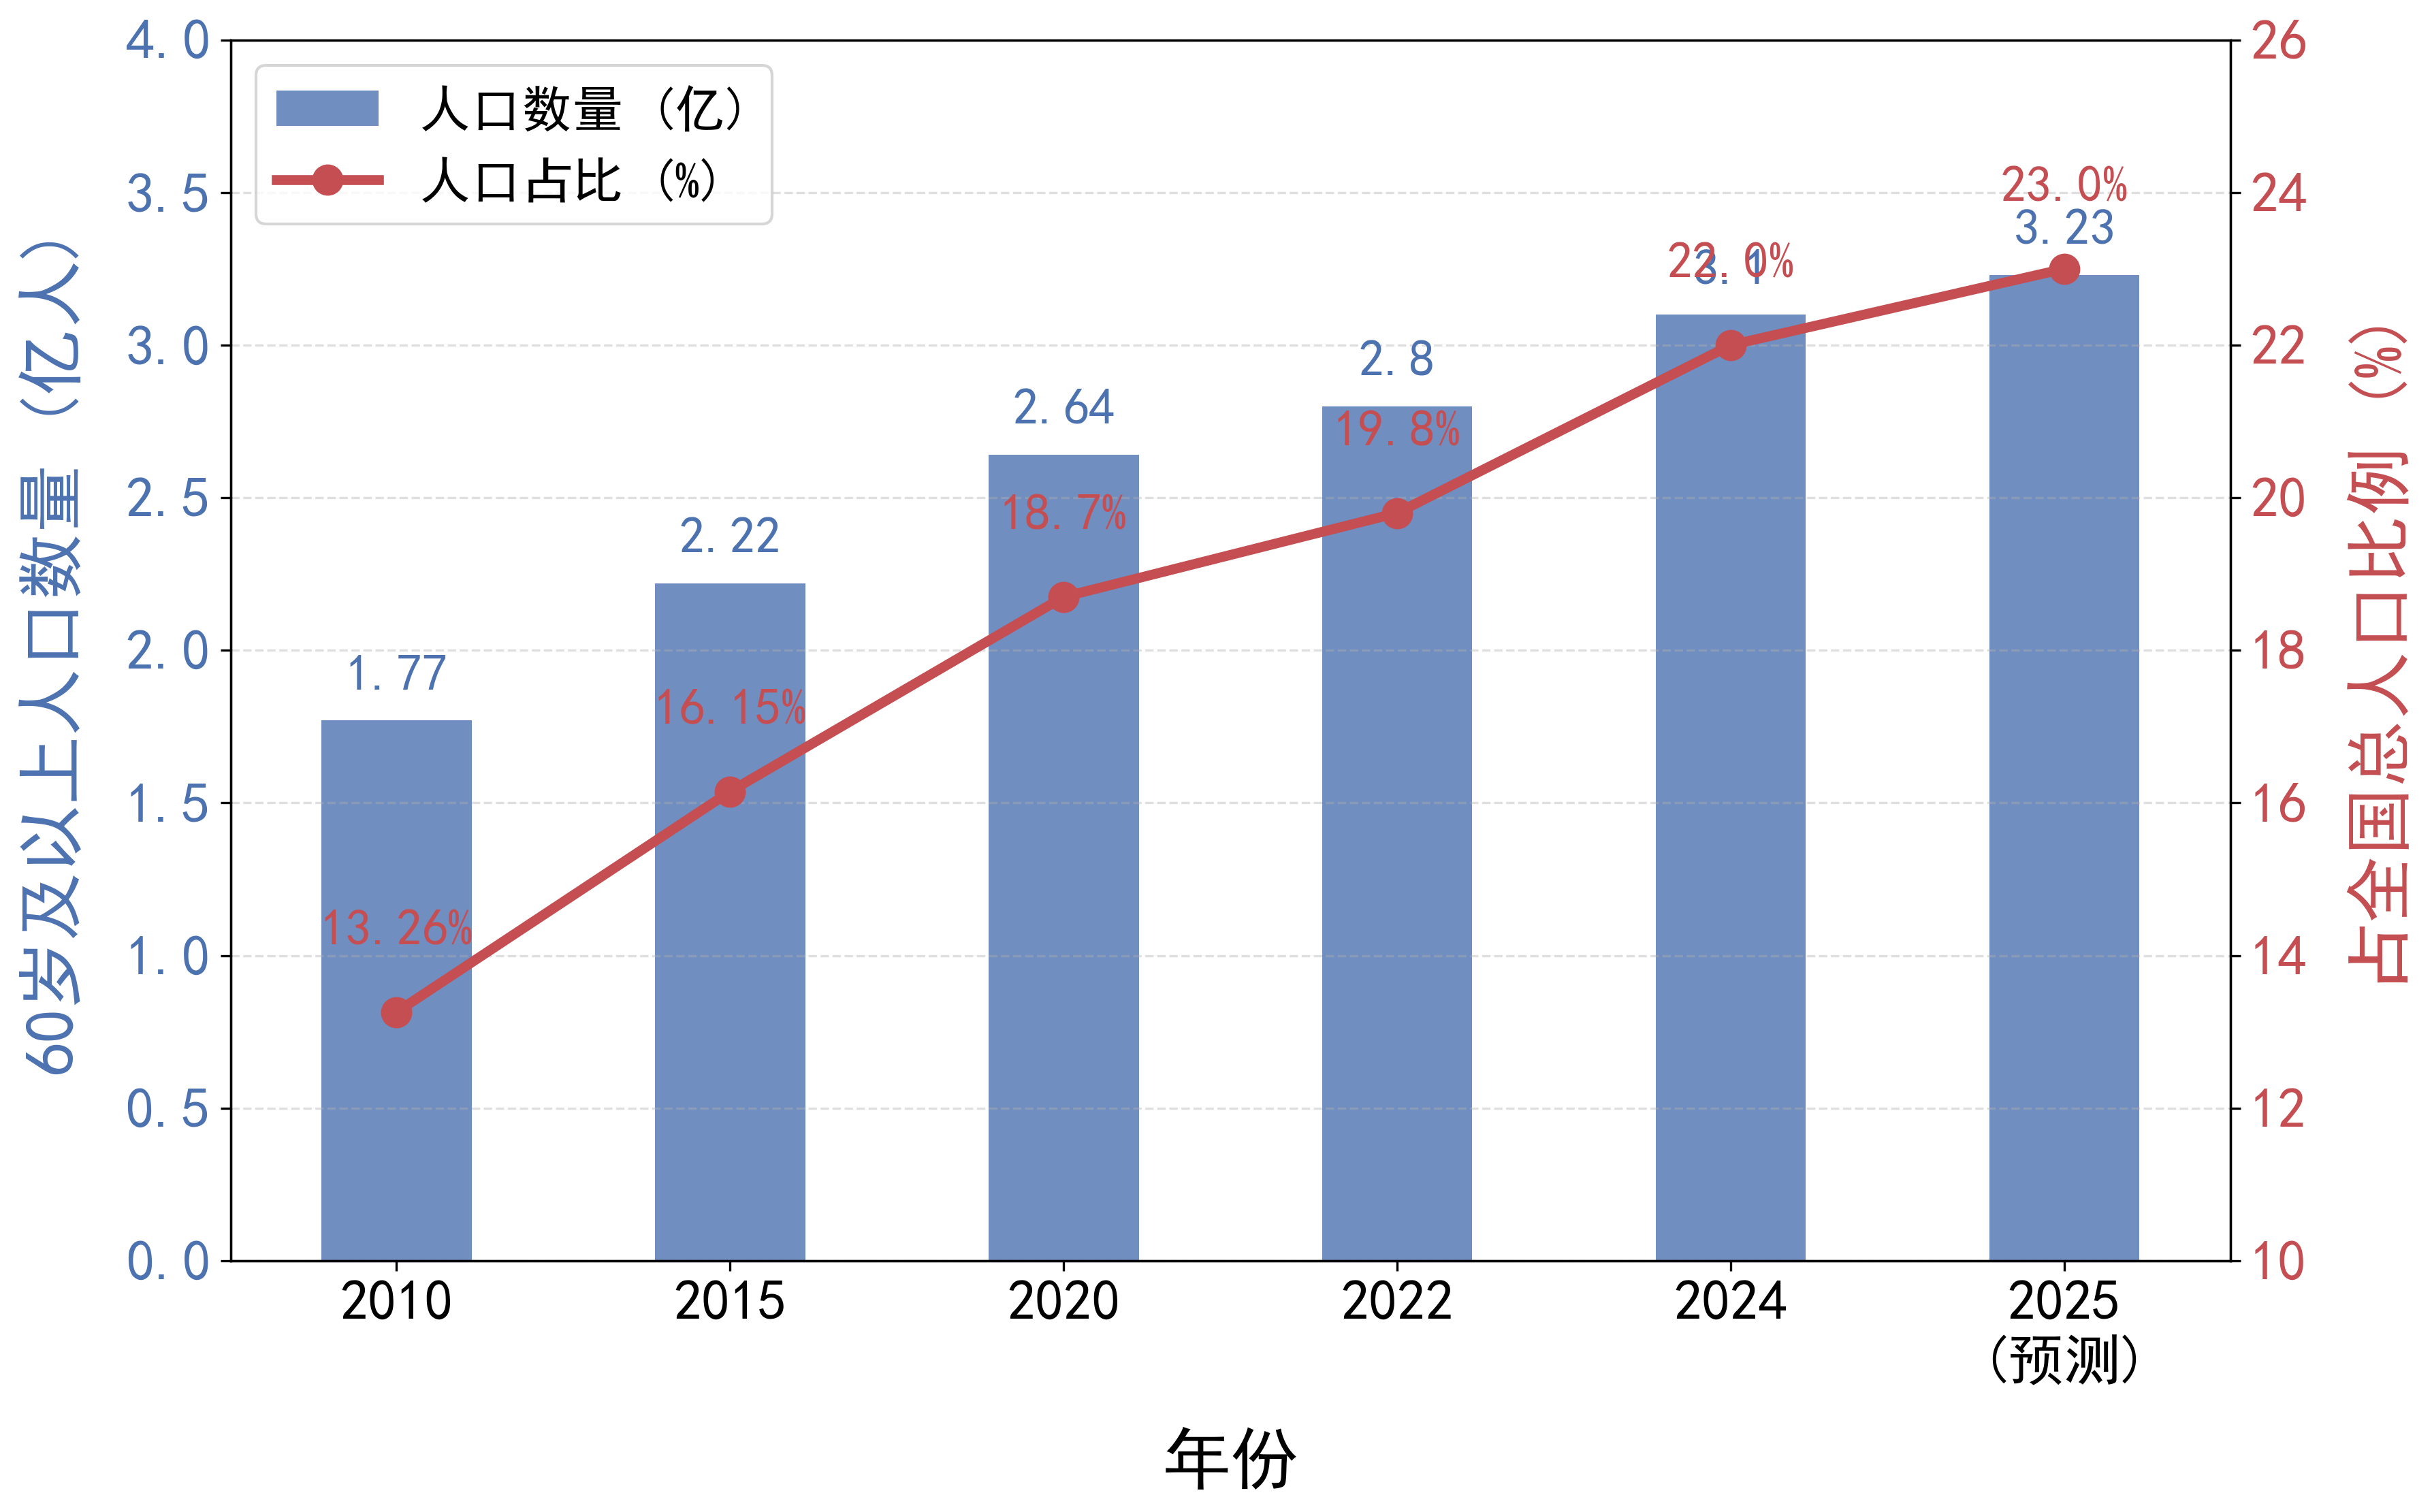
\includegraphics[width=0.85\textwidth]{figures/fig1_1_aging_population_trend.png}
    \caption{中国60岁及以上老年人口数量与占比趋势 (2010-2025)}
    \label{fig:aging_population}
\end{figure}


然而，移动终端功能的不断丰富在为大多数用户带来便利的同时，也对老年群体形成了日益突出的使用障碍。一方面，老年用户由于生理机能退化，普遍面临视力下降、听力减弱、手指灵活性降低、认知反应速度减缓等客观问题；另一方面，主流智能终端的人机交互界面设计往往以年轻用户为主要目标群体，密集的图标布局、多层嵌套的菜单结构、频繁的系统弹窗以及不断变化的应用更新，对老年人构成了显著的认知负担与操作障碍。

这种由技术快速演进与老年群体适应能力之间的差异所形成的隔阂，被学界称为“数字鸿沟”。数字鸿沟在通信领域的具体体现，包括老年人无法独立完成视频通话、容易误触系统设置导致网络中断、难以理解陌生应用界面、对授权弹窗与广告推送缺乏判断能力等。中国互联网络信息中心发布的第52次中国互联网络发展状况统计报告指出，60岁及以上网民群体占比仅为14.3\,\%\upcite{2}，远低于其在总人口中的比例，说明大量老年人在数字化浪潮中处于事实上的边缘化状态。

在通信工程专业视角下，移动通信终端不仅是数据交换的物理载体，更是承载用户与外界保持联络、获取信息、维系情感的关键媒介。如何通过终端层面的软件再设计，让老年用户重新获得对智能设备的掌控感与安全感，使其能够便捷地完成与子女的视频通话、稳定地接入家庭无线网络、流畅地使用日常应用，是当代通信工程从业者必须正视的现实命题。

\subsection{适老化痛点剖析}
从一线调研结果看，老年用户在使用主流智能手机过程中暴露出的核心痛点可归纳为以下几个方面。其一是视觉痛点，标准界面字号偏小、图标密集，导致老年人需要佩戴眼镜并凑近屏幕才能勉强辨识，长时间使用容易引发视疲劳。其二是认知痛点，多级菜单和大量弹窗使老年人难以判断当前所处的界面位置，操作过程极易迷失方向。其三是通话痛点，微信视频通话需要至少七步操作，老年人记不住流程，需要子女多次教学方能勉强掌握。其四是网络痛点，老年人误触WiFi开关后无法自行恢复连接，长时间断网而不自知，错过重要来电。其五是交互痛点，对触摸屏操作不熟练，时常出现误触或长按引发的意外操作，进一步加剧对智能设备的不安全感。

\begin{figure}[htbp]
    \centering
    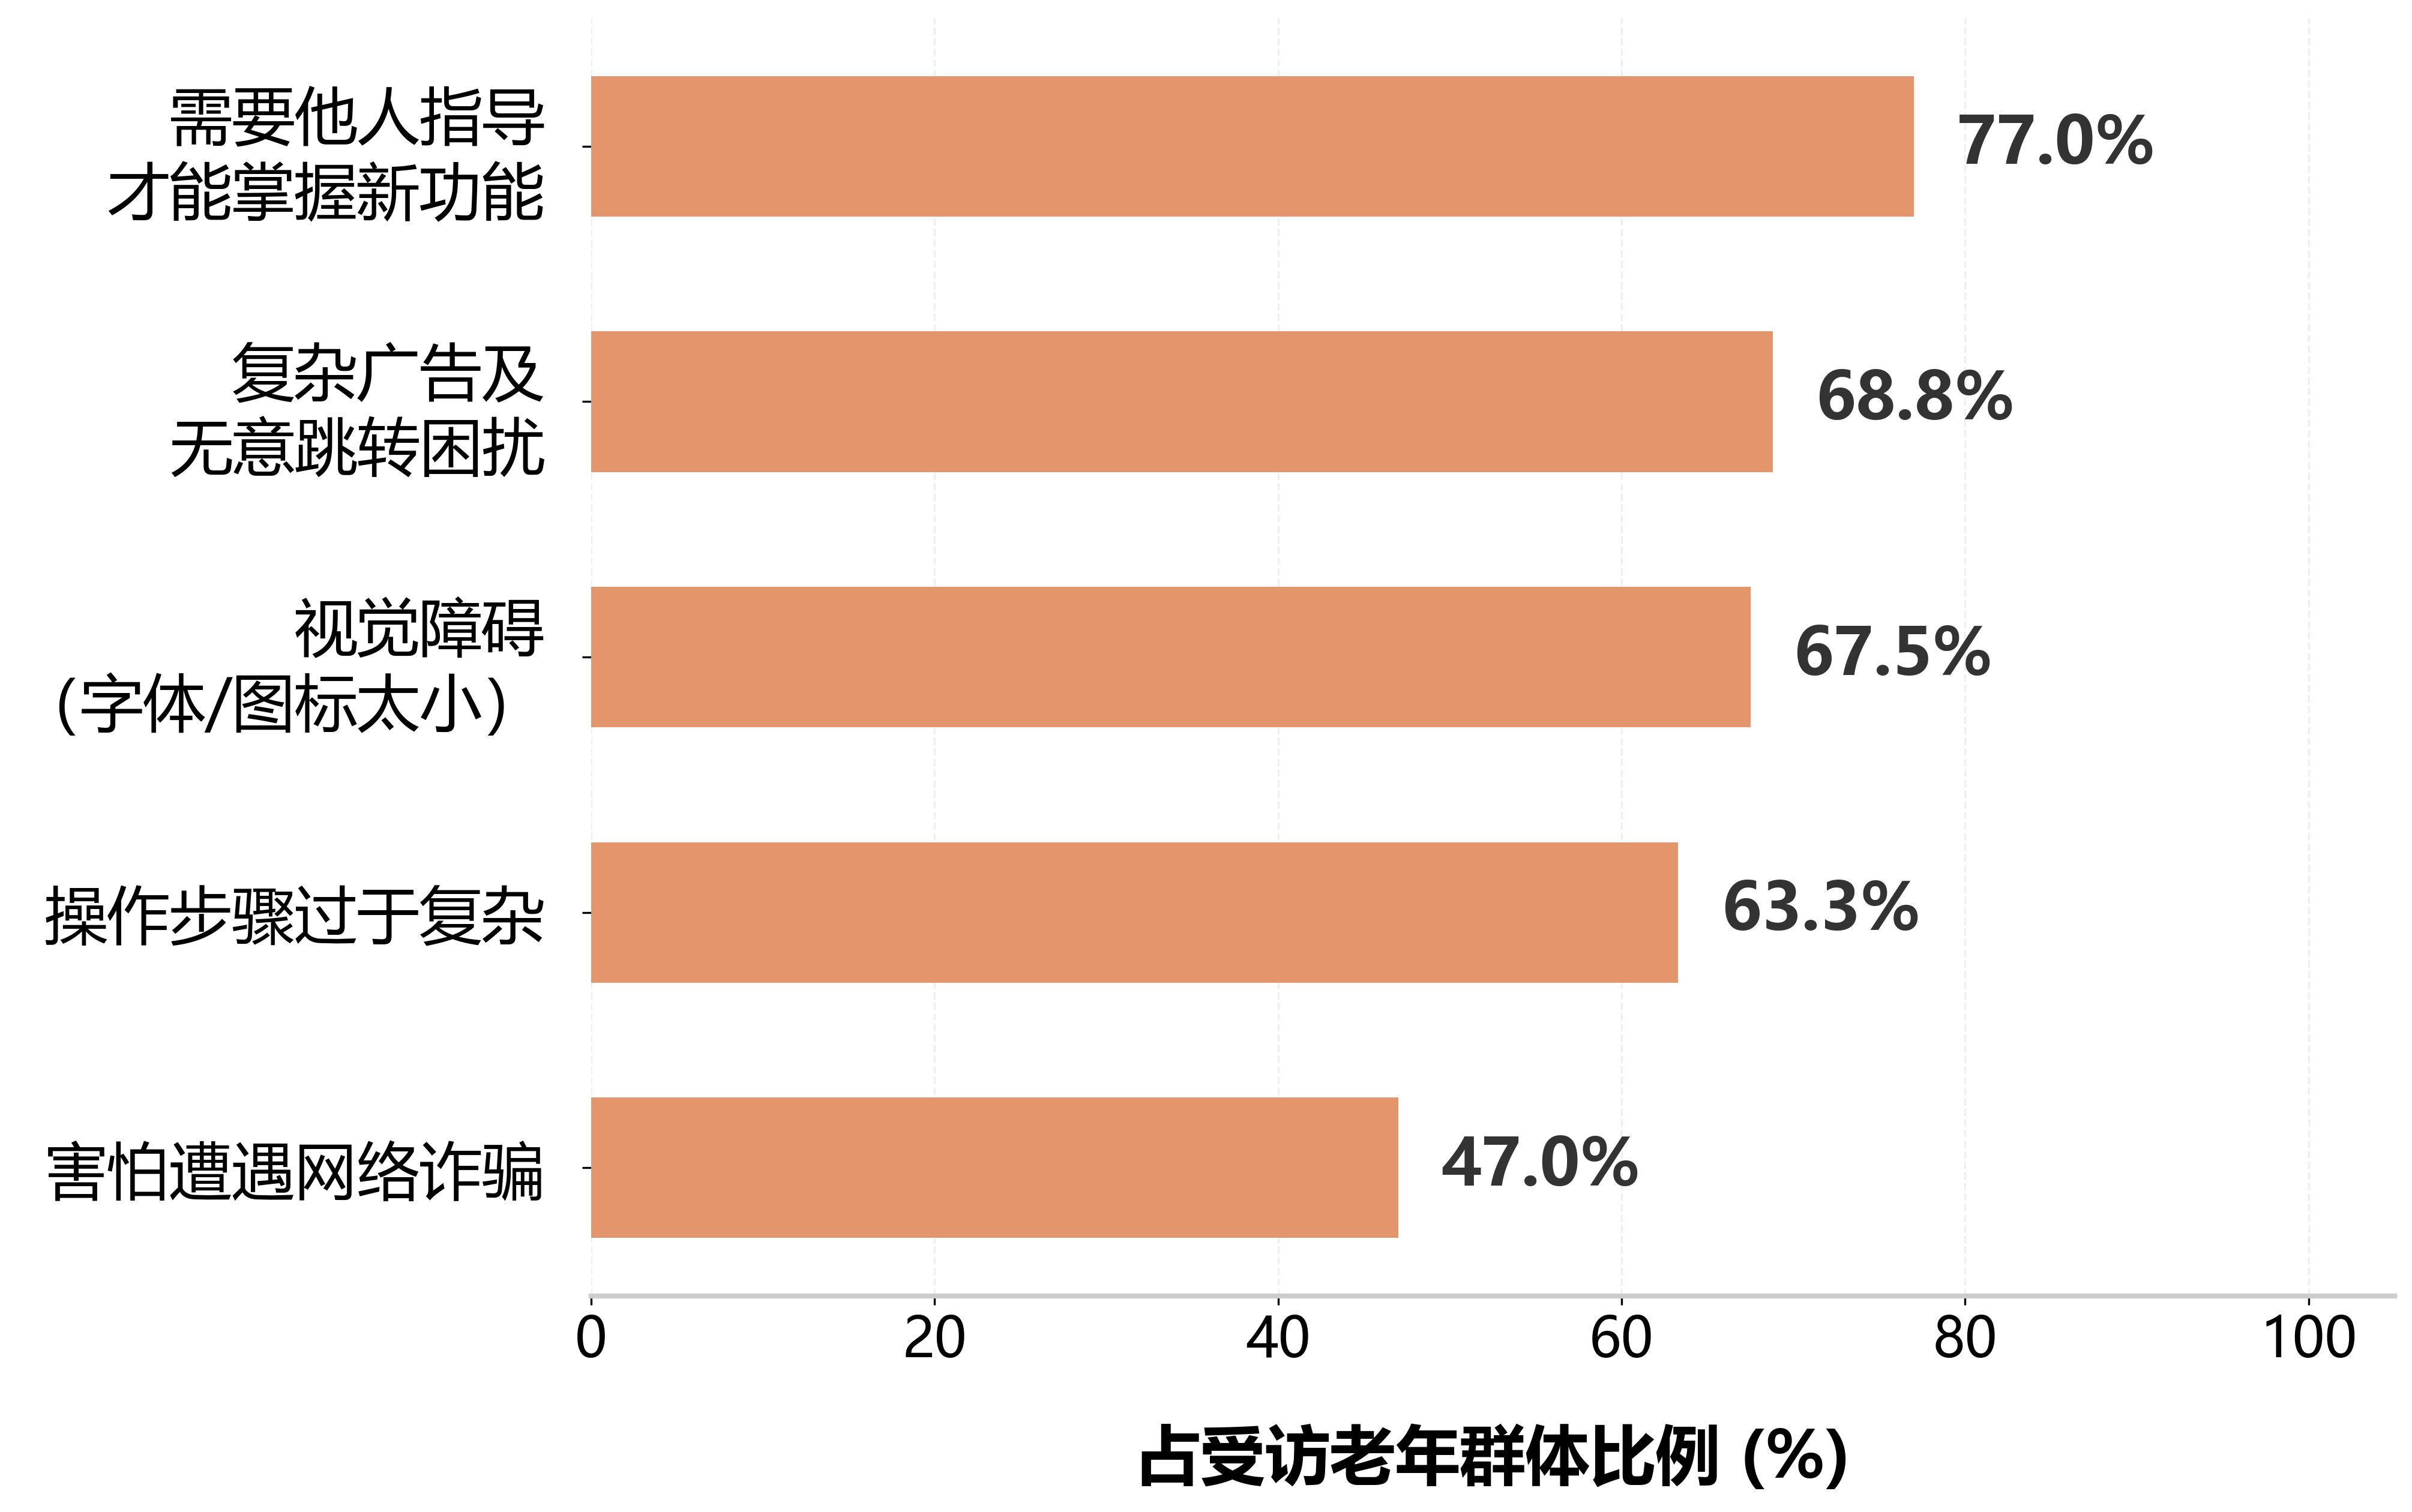
\includegraphics[width=0.85\textwidth]{figures/fig1_2_usage_pain_points.png}
    \caption{老年人智能手机使用核心痛点分布}
    \label{fig:pain_points}
\end{figure}

这些痛点的共同本质在于：现有移动通信终端的软件设计未能充分考虑老年用户的认知特征与使用习惯。仅仅通过放大字号、增大图标的浅层适老化改造，无法从根本上解决问题。必须从系统架构、交互逻辑、自动化能力等多个层面进行深度重构，才能真正为老年用户提供一款能用、好用、爱用的移动通信终端。这正是本课题立项的现实出发点。

\subsection{研究意义}
本课题以适老化智能桌面系统的设计与实现为研究对象，其意义可从社会价值、工程价值与学术价值三个维度展开。从社会价值层面看，本研究致力于通过软件技术手段帮助老年群体跨越数字鸿沟，让通信技术真正服务于全民福祉。当系统能够将原本繁琐的微信视频通话操作简化为一次点击、能够在网络异常时主动恢复并向用户清晰提示，老年用户便能更安心地依赖移动终端与家人保持联系，独居老人的精神慰藉与紧急求助通道也得到了实质性保障，这对于构建友好型老龄化社会具有积极意义。

从工程价值层面看，本课题摒弃了传统适老化方案“放大字号、堆叠图标”的简单做法，转而从系统架构与人机交互两个维度同步发力。通过自研的微内核插件化架构，系统在功能扩展性与运行稳定性方面取得了良好平衡，能够适配从千元入门机到主流旗舰机型的多种硬件配置；通过Android无障碍服务深度整合的微信一键直拨方案，系统从交互层面真正消除了老年用户的认知负担，为同类终端应用的设计提供了可复用的工程范式。

从学术价值层面看，本研究在通信终端无障碍交互、跨应用自动化控制、网络稳定性自愈等方向进行了有益探索。所提出的七阶段状态机驱动的自动化控制模型、双通道节点检索方法以及分层防御的网络守护机制，丰富了适老化通信终端研究的理论与实践成果，对推动我国老年友好型移动通信生态建设具有借鉴意义。

% \section{国内外研究现状}

% \subsection{移动通信终端适老化研究现状}
% 终端适老化是一个跨越通信工程、人机交互、工业设计、认知心理学等多学科的综合性研究方向。从国际范围来看，欧美国家由于步入老龄化社会较早，相关研究起步亦较早。日本与德国的研究机构较早提出了“通用设计”与“包容性设计”理念，主张通过通用化的界面与功能设计兼顾各年龄段用户的使用需求。在产品形态上，海外市场早年出现了Doro、Jitterbug等专注于老年用户的终端品牌，以及Big Launcher、Simple Launcher等第三方桌面应用，其设计思路普遍以大尺寸瓷砖式布局取代传统的网格图标布局，并精简非必要功能入口。近年来，国际厂商的适老化策略逐渐向系统原生辅助功能演进。然而，海外方案在中国本土的适用性较为有限，例如其无法对国内老年用户高度依赖的微信、支付宝等超级应用进行深度适配，也难以兼容中国传统农历、节气等本土文化要素。

% 国内方面，伴随老龄化进程的加快和工信部“互联网应用适老化及无障碍改造”专项行动\upcite{3}的持续推进，主流手机厂商相继推出了系统级适老化方案。华为的“简易模式”、小米的“极简模式”、OPPO的“简单模式”以及荣耀的“长辈模式”等，均对系统字号、图标尺寸、铃音音量等进行了适当优化，并在拦截骚扰电话、识别诈骗短信等方面提供了一定支持。但当前阶段，这些厂商方案的共同局限在于，其作用范围仅限于操作系统层面，无法越权穿透至第三方应用内部。换言之，老年用户进入微信、支付宝等具有复杂层级架构的具体应用后，依然需要面对其原生的复杂交互逻辑，由于认知负荷增加，操作障碍并未得到根本解决，跨应用的“数字鸿沟”依然显著。

% \begin{figure}[htbp]
%     \centering
%     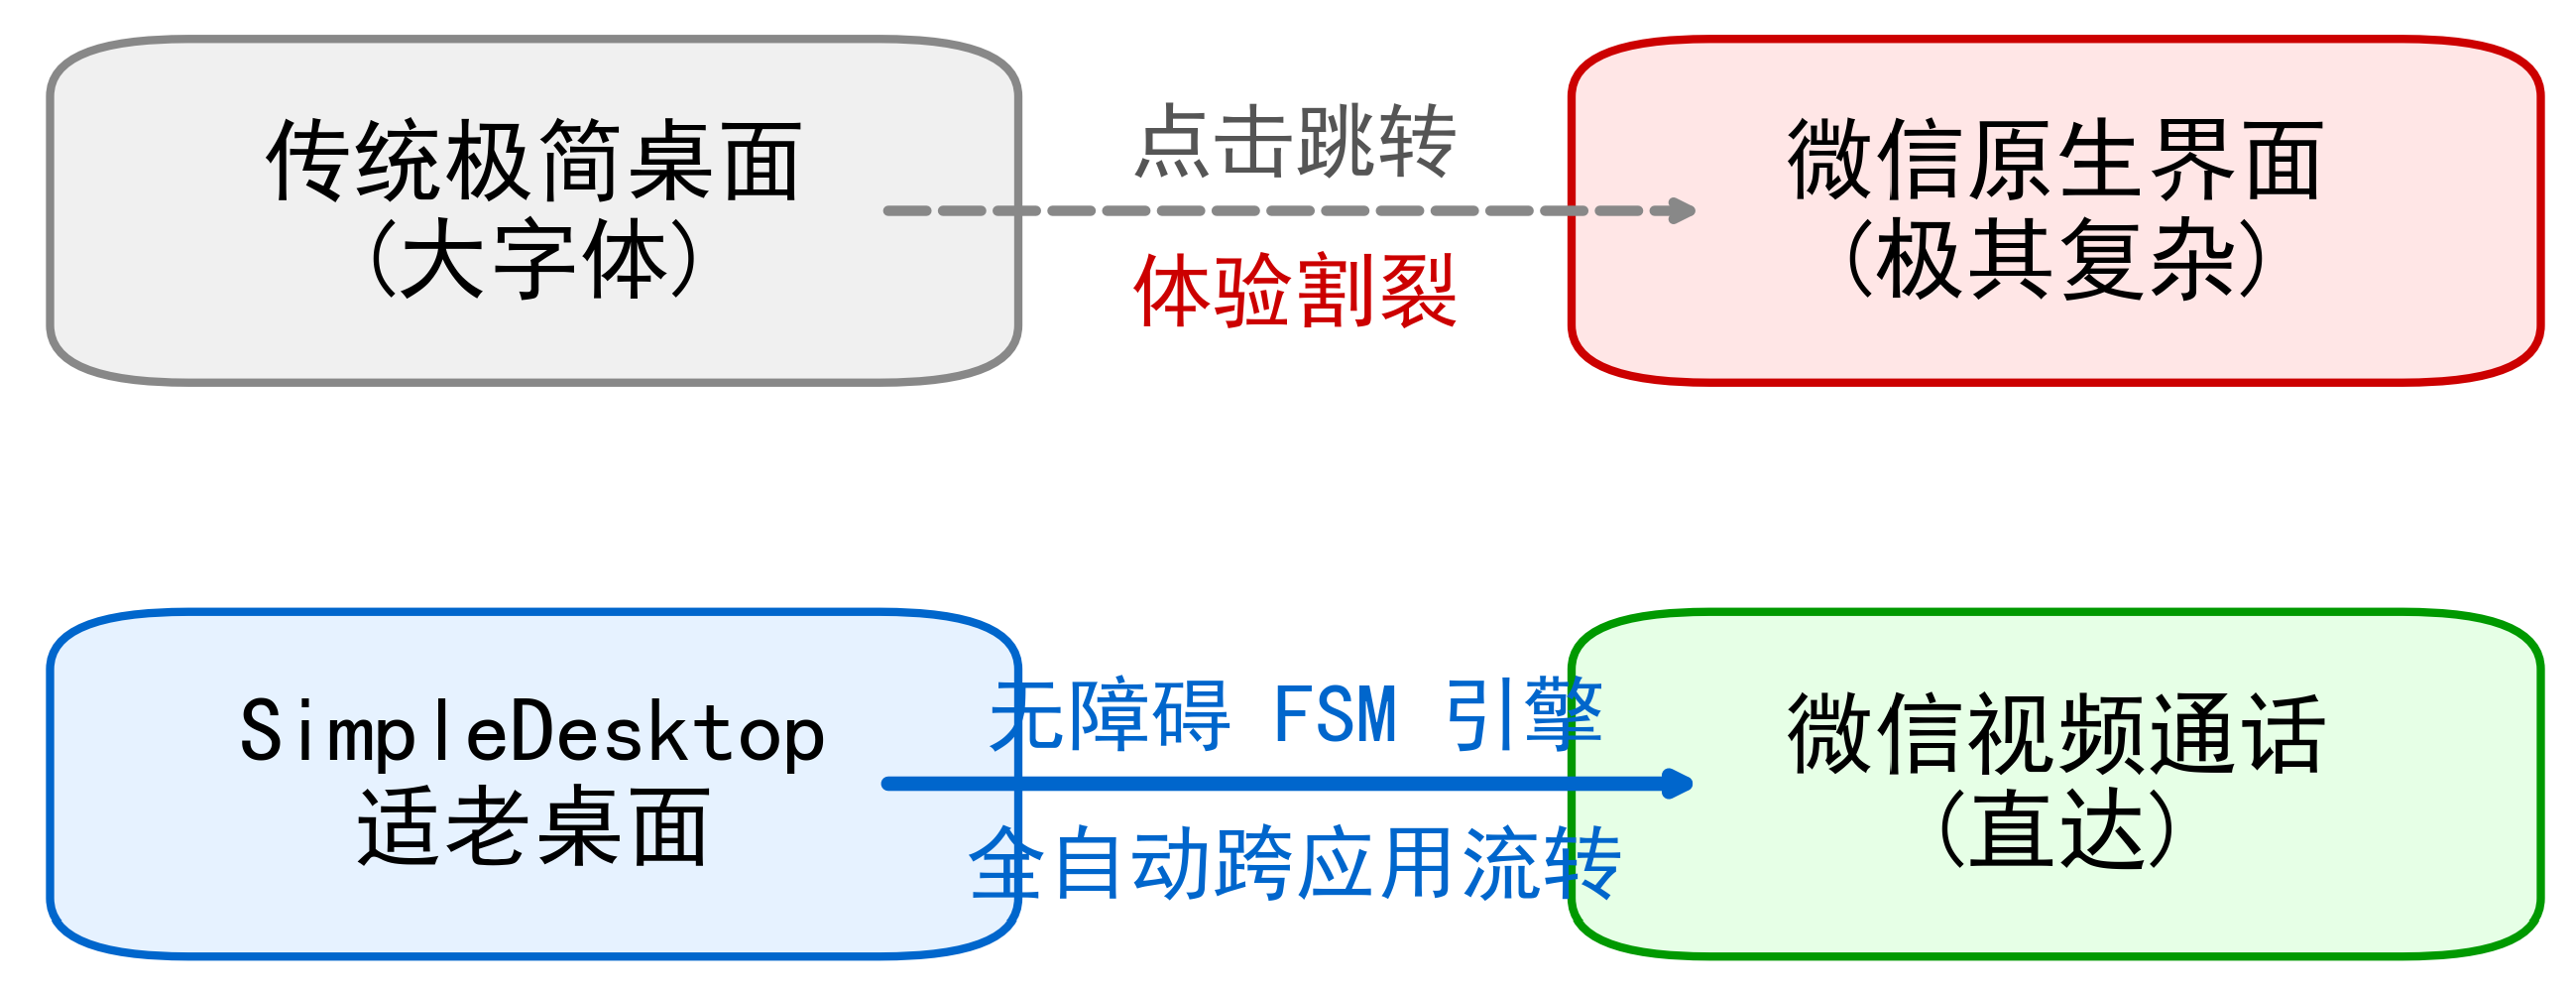
\includegraphics[width=0.9\textwidth]{figures/fig1_3_architecture_compare.png}
%     \caption{传统适老化桌面与本系统自动化直达通道的体验对比}
%     \label{fig:arch_compare}
% \end{figure}

% 在学术研究方面，近年来国内外学者围绕适老化终端开展了多方面探索。文献研究普遍聚焦于以下三个方向：一是基于Fitts定律的触控目标尺寸优化，从生理人因学角度论证大按钮设计的合理性；二是基于对比敏感度模型的色彩搭配研究，提出适合老年视觉特征的高对比度配色方案；三是基于眼动追踪与认知负荷模型的界面可用性评估，验证简化界面对老年用户操作效率的提升效果。然而，相关研究多聚焦于界面表层的视觉与布局优化\upcite{4-6}，鲜有研究涉及如何突破应用壁垒，让老年人在第三方应用内部也能享受到简化体验这一深层次工程命题\upcite{8}。

% \subsection{Android无障碍自动化技术研究现状}
% 要实现跨第三方应用的操作简化，业界普遍采用Android平台提供的无障碍服务（Accessibility Service）作为技术抓手。相较于需要底层调试权限的自动化测试框架，无障碍服务因其伴随系统安全运行的特性，成为端侧辅助控制的首选。该服务最初是为视障用户提供屏幕朗读功能而设计的系统级接口，但因其具备读取屏幕控件树和执行模拟操作的能力，近年来被广泛应用于自动抢红包、自动签到、自动化测试等多种场景。

% 从已有的研究与产品实践来看，基于无障碍服务的自动化控制方案主要存在以下不足：首先，绝大多数实现方式依赖目标应用控件的资源标识符进行硬编码定位，一旦目标应用版本更新、启用代码混淆，或采用跨平台前端框架导致控件树不透明，自动化流程便会迅速失效\upcite{7}；其次，缺乏对系统级弹窗、来电中断等异常情况的时序容错处理机制，导致流程稳定性较差；再次，普遍缺乏对老年用户场景的针对性优化，未能将自动化能力转化为面向终端用户的简洁可靠服务。

% 从最近的发展趋势来看，随着人工智能技术的爆发，基于视觉-语言模型（VLM）的图形用户界面智能体（GUI Agent）成为了无障碍自动化的前沿热点。研究者试图跳出底层控件树的限制，直接通过计算机视觉结合大模型逻辑推理，实现自然语言驱动的UI自动化操作。这类技术在应对应用更新方面展现了巨大潜力。然而，大模型驱动的自动化目前仍面临端侧算力消耗大、推理延迟高且强依赖云端网络等瓶颈，难以直接部署在计算资源普遍有限的适老机型上作为实时守护服务。

% 综合上述现状可知，尽管移动终端适老化已取得一定进展，但“第三方应用内部操作门槛高”与“现有自动化方案稳定性差”之间仍存在巨大体验断层。在通信终端无障碍交互方向上，既有研究多关注屏幕朗读、语音输入等输入输出层面的辅助技术，对于如何利用无障碍能力构建稳定可靠的跨应用通信桥接这一问题，缺乏系统性的工程方案。本课题正是着眼于这一研究空白，放弃脆弱的线性脚本硬编码方案，探索通过状态机建模、双通道检索、焦点退避等多级容错机制，构建具备较高鲁棒性的适老化终端自动化通信能力，从而真正将底层的无障碍能力转化为老年用户一触即达的极简体验。

\section{国内外研究现状}

\subsection{移动通信终端适老化研究现状}
终端适老化是一个跨越通信工程、人机交互、工业设计、认知心理学等多学科的综合性研究方向，其核心目标是通过软件与硬件层面的协同优化，消除老年用户与智能终端之间的交互障碍。从国际范围来看，欧美国家由于步入老龄化社会较早，相关研究起步亦较早。日本与德国的研究机构在20世纪90年代便较早提出了"通用设计"（Universal Design）与"包容性设计"（Inclusive Design）理念\upcite{4}，主张通过统一化的界面与功能规范兼顾各年龄段用户的使用需求，而非为老年群体单独构建隔离式的特殊产品。在产品形态上，海外市场早年出现了Doro、Jitterbug等专注于老年用户的简化功能终端品牌，以及Big Launcher、Simple Launcher等第三方桌面替换应用。其设计核心思路是以大尺寸瓷砖式布局取代传统网格图标，将最常用的通话、短信、紧急求助等入口直接置于主界面，并通过提升触控目标尺寸降低误触率。研究表明，将触控目标直径从标准的7mm增大至13mm以上，可使老年用户的操作出错率降低约38\%\upcite{5}。近年来，国际主流厂商的适老化策略逐渐向系统原生辅助功能演进，Apple iOS的"辅助功能"（Accessibility）模块、Google Android的无障碍框架均持续扩充字体缩放、高对比度显示、触控辅助等能力体系。

然而，上述海外方案在中国本土的适用性较为有限。一方面，其无法对国内老年用户高度依赖的微信、支付宝、健康码等超级应用进行深度交互适配，用户仍需自行应对这些应用复杂的内部操作逻辑；另一方面，海外方案亦难以兼容农历纪年、传统节气提示、国内紧急呼救号码体系等中国本土文化与服务要素，致使其无法直接满足国内老年群体的实际需求。

国内方面，伴随老龄化进程的加快和工信部"互联网应用适老化及无障碍改造"专项行动\upcite{3}的持续推进，主流手机厂商相继推出了系统级适老化方案，形成了一定的产业实践积累。华为的"简易模式"、小米的"极简模式"、OPPO的"简单模式"以及荣耀的"长辈模式"等，均对系统桌面字号、图标尺寸、铃音音量等进行了适当优化，并在拦截骚扰电话、识别诈骗短信等安全场景提供了初步支持。部分厂商还针对老年用户推出了专属内容频道与亲情账号绑定功能，尝试从内容与服务维度实现适老化延伸。

然而，上述厂商方案的共同局限在于，其适老化能力的作用边界止步于操作系统的桌面启动层（Launcher）。当老年用户进入微信、支付宝等具有深度层级架构的第三方应用后，依然需要独立面对其原生的多级菜单、频繁弹窗与细小控件，认知负荷未得到实质性缓解。以微信视频通话为例，从桌面出发到拨通视频电话，标准流程最少需经历"打开微信→进入通讯录→定位联系人→进入会话→点击视频通话→二次确认"共六至七步操作，对于认知能力下降的老年用户而言，这一操作链极易在任意环节发生中断\upcite{6}。由此可见，当前适老化实践存在明显的"系统层优化充分、应用层穿透不足"的结构性断层，跨应用层面的"数字鸿沟"依然显著。

\begin{figure}[htbp]
    \centering
    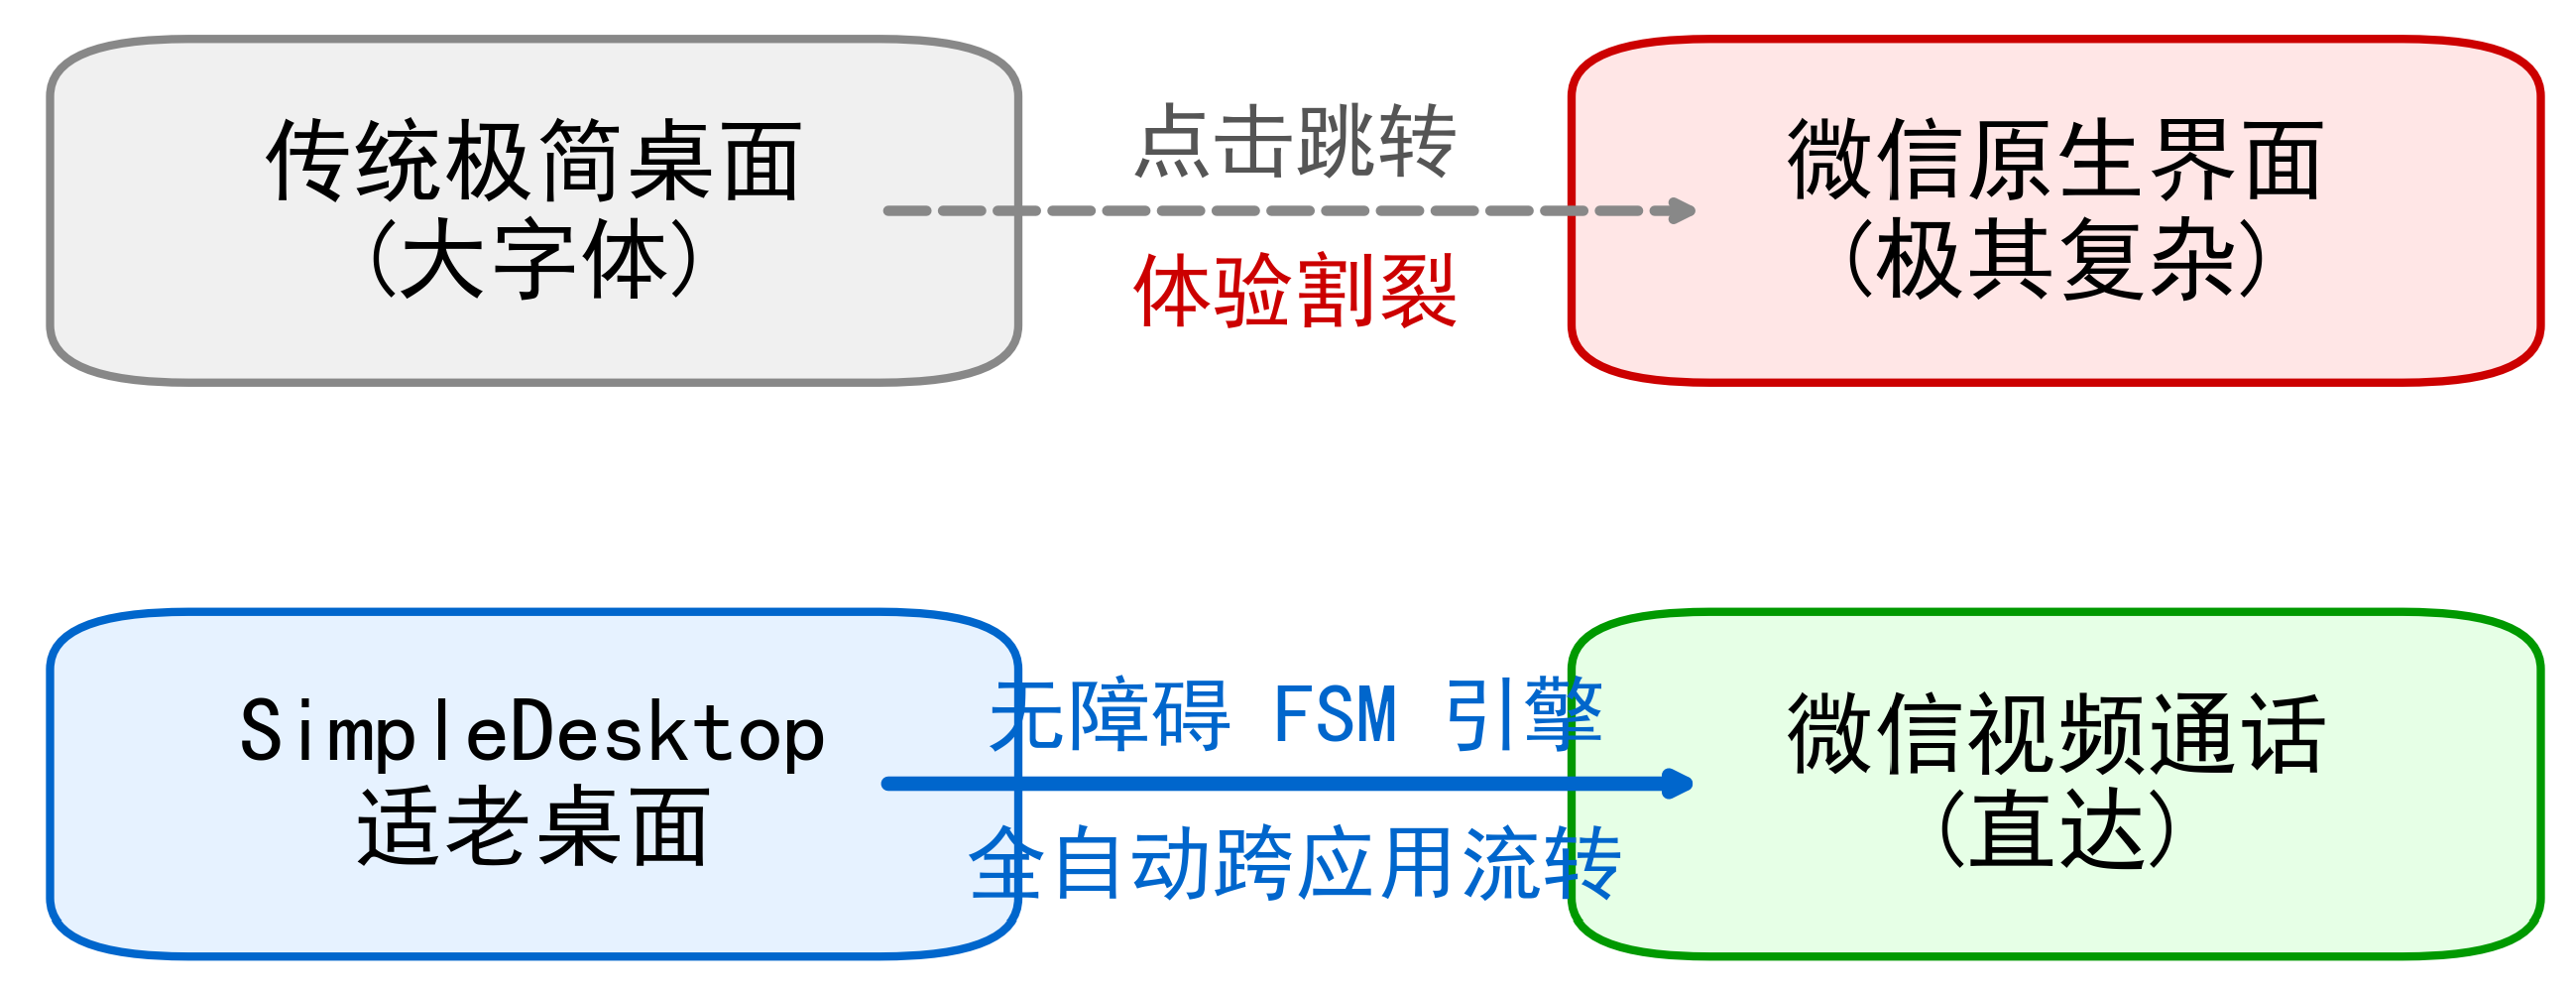
\includegraphics[width=0.9\textwidth]{figures/fig1_3_architecture_compare.png}
    \caption{传统适老化桌面与本系统自动化直达通道的体验对比}
    \label{fig:arch_compare}
\end{figure}

在学术研究层面，近年来国内外学者从多个维度围绕适老化终端展开了探索。在人因工程方向，研究者基于Fitts运动定律对老年人触控行为建立了量化模型，系统论证了增大触控目标面积与降低界面元素密度对提升操作精度的正向作用；在视觉认知方向，依据对比敏感度函数（Contrast Sensitivity Function）建立的色彩可读性评估模型，为适老配色标准的制定提供了理论依据，相关研究指出前景与背景的WCAG对比度比值维持在4.5:1以上可显著改善老年用户的文字识别率；在可用性工程方向，综合眼动追踪数据与NASA-TLX认知负荷量表的实验研究验证了界面层级简化对老年用户任务完成效率的积极影响\upcite{5,6}。

尽管如此，上述研究均聚焦于终端界面的视觉呈现与信息架构优化，较少涉及如何在保持原生应用界面不变的前提下，通过系统层的技术介入为老年用户构建更短的操作路径\upcite{8}。这一跨应用穿透与代理执行的深层次工程命题，在已有文献中尚属显著研究空白，也是本课题在现有适老化研究基础上谋求突破的核心切入点。

\subsection{Android无障碍自动化技术研究现状}
要在不修改第三方应用源码的前提下实现跨应用的操作简化，业界和学界普遍将Android平台提供的无障碍服务（AccessibilityService）视为最具可行性的技术抓手。无障碍服务是Android系统为辅助视障、肢障等特殊用户群体而设计的系统级接口，其核心能力包括：订阅并接收全局窗口内容变化、焦点切换等辅助事件，通过控件信息对象（AccessibilityNodeInfo）遍历当前界面的完整视图树（View Tree），以及向目标控件派发模拟点击、长按、文本输入、手势滑动等操作指令。由于无障碍服务随系统进程安全运行，无需root权限或USB调试连接，相较于UIAutomator等需要底层特权的自动化测试框架，其在消费级终端上的部署可行性更高，因此被广泛用于自动抢红包、自动打卡签到、辅助输入等商业场景。

然而，从已有研究与工程实践来看，当前基于无障碍服务的自动化控制方案普遍存在三方面结构性缺陷。其一是跨版本稳定性差。绝大多数实现依赖目标应用控件的静态资源标识符（Resource-ID）进行硬编码定位，一旦目标应用进行版本迭代并启用R8/ProGuard代码混淆，或底层改用Flutter、React Native等跨平台框架造成原生控件树不透明，原有定位逻辑即告失效\upcite{7}。微信作为持续高频迭代的超级应用，平均每两至三个月发布一次影响内部控件结构的大版本更新，这对硬编码方案构成了持续性的维护压力。其二是时序容错能力薄弱。现有方案多采用固定延时的线性脚本逻辑，对页面加载速度受设备性能与网络状况动态影响的客观规律缺乏适应性处理，对来电中断、系统权限弹窗、屏幕旋转等外部事件亦无动态感知与流程自恢复机制，导致在真实老年用户的复杂使用环境中流程稳定性严重不足。其三是缺乏老年场景的专项适配。已有研究与产品将无障碍服务视为开发者调试工具，而非面向终端老年用户的可靠产品能力，对老年人误触屏幕、场景切换频繁导致的焦点争抢（Focus Competition）等特殊问题缺乏针对性的防护设计，极易造成自动化流程陷入死锁。

从技术演进前沿来看，随着多模态大语言模型（Multimodal LLM）的快速发展，基于视觉-语言模型（Vision-Language Model，VLM）的图形用户界面智能体（GUI Agent）已成为无障碍自动化领域的前沿研究热点。此类方案通过对屏幕截图进行视觉理解，结合大模型的逻辑推理能力，以自然语言指令驱动跨应用自主导航，从理论上摆脱了对底层控件树结构的硬编码依赖，具备较强的跨版本泛化潜力。然而，现阶段大模型驱动的GUI自动化在端侧部署方面仍面临不可回避的工程瓶颈：典型的多模态推理模型参数量超过70亿，端侧运行显存需求通常在8GB以上，在主流适老化目标机型（中低端Android设备）上无法实现实时响应；同时，强依赖云端API调用引入了不可控的网络延迟，而老年用户的网络环境本身往往是系统需要主动守护的脆弱环节，两者形成悖论。

综合上述研究现状可以判断，尽管移动终端适老化与无障碍自动化两个方向均已取得一定进展，但"第三方应用内操作门槛高"与"现有端侧自动化方案跨版本稳定性差"之间依然横亘着显著的技术鸿沟。在通信终端无障碍交互方向，既有研究多聚焦于屏幕朗读、语音输入等单向辅助技术，对于如何利用无障碍能力主动代理老年用户完成微信通话等高频复杂操作，并保证在真实环境下的鲁棒性这一问题，缺乏系统性的工程方法论。本课题正是着眼于这一研究空白，放弃依赖Resource-ID的硬编码脆弱路径，提出并实现了以七阶段状态机建模、双通道节点检索、焦点退避与心跳防死锁为核心的多级容错自动化框架，以期在无需云端大模型支撑、无需设备特殊权限的前提下，为老年用户提供稳定、低延迟、跨版本兼容的一键直拨通信能力。



\section{主要研究内容}
针对前述移动通信终端在适老化方向上的痛点和现有研究的不足，本课题完成了一款面向老年用户的Android智能桌面系统SimpleDesktop的全栈设计与实现。系统以问题驱动为基本思路，围绕老年用户实际遇到的视觉障碍、操作障碍、通话障碍、网络障碍和交互障碍五大问题，相应展开五个方向的研究与实践。

一是面向终端架构稳定性的微内核插件化引擎研究。系统摒弃了传统单体式应用架构，将桌面信息聚合、联系人通讯、应用启动、天气服务等业务功能解耦为相互独立的功能插件，并通过统一的插件管理器和消息总线进行协调。该架构既保证了系统在低端设备上的稳定运行，也为未来扩展健康监测、智能家居控制等模块预留了清晰接口。

二是面向老年视觉与认知特征的适老化人机交互界面研究。系统基于现代声明式UI框架构建了高对比度、大字号、卡片化的桌面界面规范，支持不同字号档位与多种主题方案的实时切换，并在主屏中以聚合面板的形式集中呈现时间、农历、天气、常用联系人和常用应用，最大限度降低老年用户的视觉搜索成本。

三是面向无障碍通信的微信一键自动通话研究。针对老年用户使用微信视频通话操作步骤过多的问题，提出基于Android无障碍服务的七阶段状态机自动化方案\upcite{24,26}，配合双通道节点检索算法\upcite{30}和焦点防冲突退避机制\upcite{29}，实现桌面点击联系人、系统自动完成全部微信操作、直接进入视频通话的一键化流程。

四是面向终端通信连续性的WiFi网络守护研究。系统通过常驻前台服务持续监测网络连接状态，一旦检测到WiFi断连便进入宽限期等待自动恢复；超过宽限期后，借助无障碍服务自动开启WiFi开关，并通过弹窗与语音播报双重通道引导用户进行必要的人工干预，从而最大限度保障通信链路的连续性。

五是面向自然语言交互的语音助手研究。系统基于Android原生TTS引擎实现全局语音播报，并通过关键词匹配与编辑距离容错相结合的轻量级语义解析方法\upcite{13}，将打电话给某某等自然语言指令准确映射到具体的通信操作上，使老年用户无需依赖屏幕触控即可完成主要操作。

\begin{figure}[htbp]
    \centering
    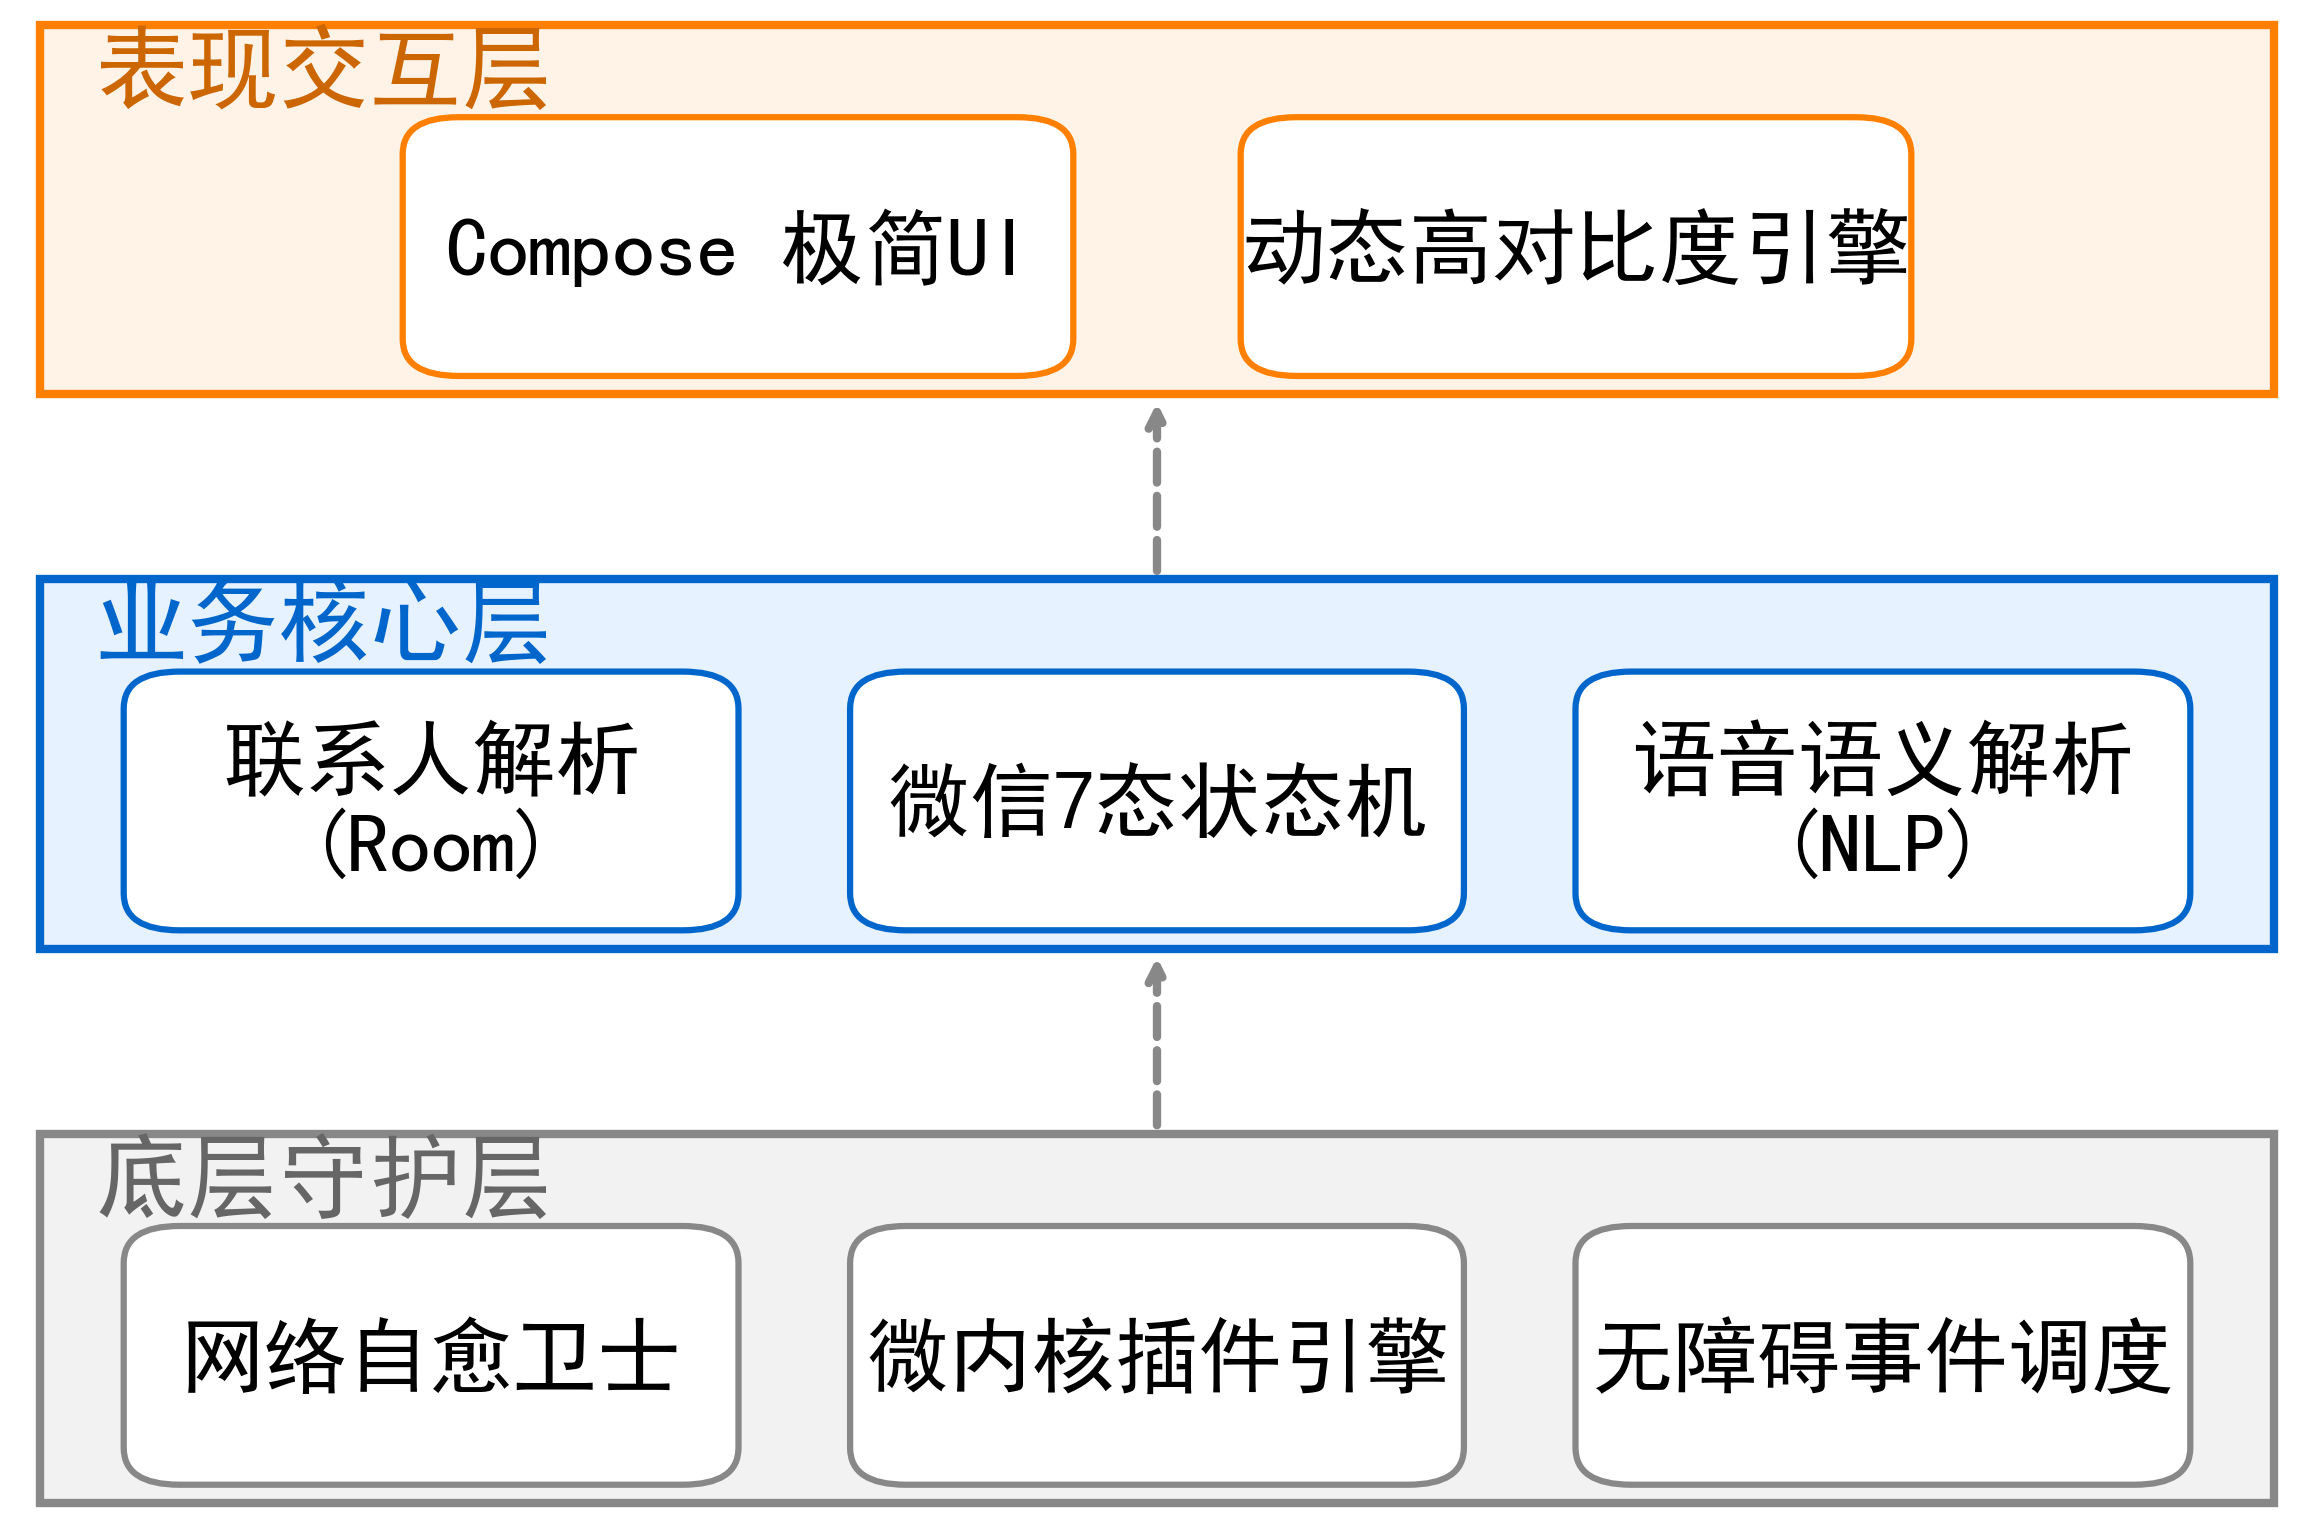
\includegraphics[width=0.9\textwidth]{figures/fig1_4_system_overview.png}
    \caption{SimpleDesktop 系统技术全景架构图}
    \label{fig:system_overview}
\end{figure}

\section{论文组织结构}
全文共分五章，各章主要内容如下。

第1章为绪论，主要介绍课题的研究背景、研究意义、国内外研究现状、主要研究内容以及论文的组织结构，旨在明确研究的出发点与全文的整体脉络。

第2章为技术基础，主要介绍本课题所依赖的技术体系，包括现代Android技术栈、数据持久化与依赖注入框架、微内核插件化架构理论以及Android无障碍服务的基本原理，为后续章节的设计与实现奠定理论与技术基础。

第3章为适老化智能桌面系统的设计与实现，是论文的核心章节。首先从老年用户视角出发开展需求分析，然后给出宿主层、总线层、插件层三层架构的整体设计方案并交代开发环境，接着分别对适老化界面、微信自动化直连、WiFi网络守护、语音辅助等核心功能模块进行设计与实现的详细阐述，最后给出软件的整体操作流程。

第4章为软件测试与分析，依次从功能测试、兼容性测试和性能测试三个维度对系统质量进行系统化评估。功能测试覆盖联系人增删改查、应用管理、微信通话发起、语音指令解析等核心用例；兼容性测试覆盖不同型号、不同分辨率、不同系统版本的真机环境；性能测试关注响应时间、页面加载速度以及多并发访问的处理能力。

第5章为总结与展望。首先对全文工作进行总结，凝练课题的主要成果与贡献；其次客观分析当前系统存在的局限性，并对未来的研究方向作出展望。









































\iffalse

\chapter{绪论}
\section{研究背景与意义}
\subsection{人口老龄化加剧下的移动通信终端使用困境}
伴随我国人口结构的深刻变化，老龄化已成为关乎国计民生的重要社会议题。根据国家统计局发布的数据，截至2023年末，我国60岁及以上人口已达2.97亿，占总人口的21.1\,\%\upcite{1}，预计到2035年这一比例将突破30\%，我国正稳步迈向中度老龄化社会。在通信技术高速发展的背景下，移动通信终端早已超越传统的语音通话功能，演变为集即时通讯、移动支付、远程医疗、出行导航等多重服务于一体的综合数字生活入口，深度融入了现代社会的各个角落。


\begin{figure}[htbp]
    \centering
    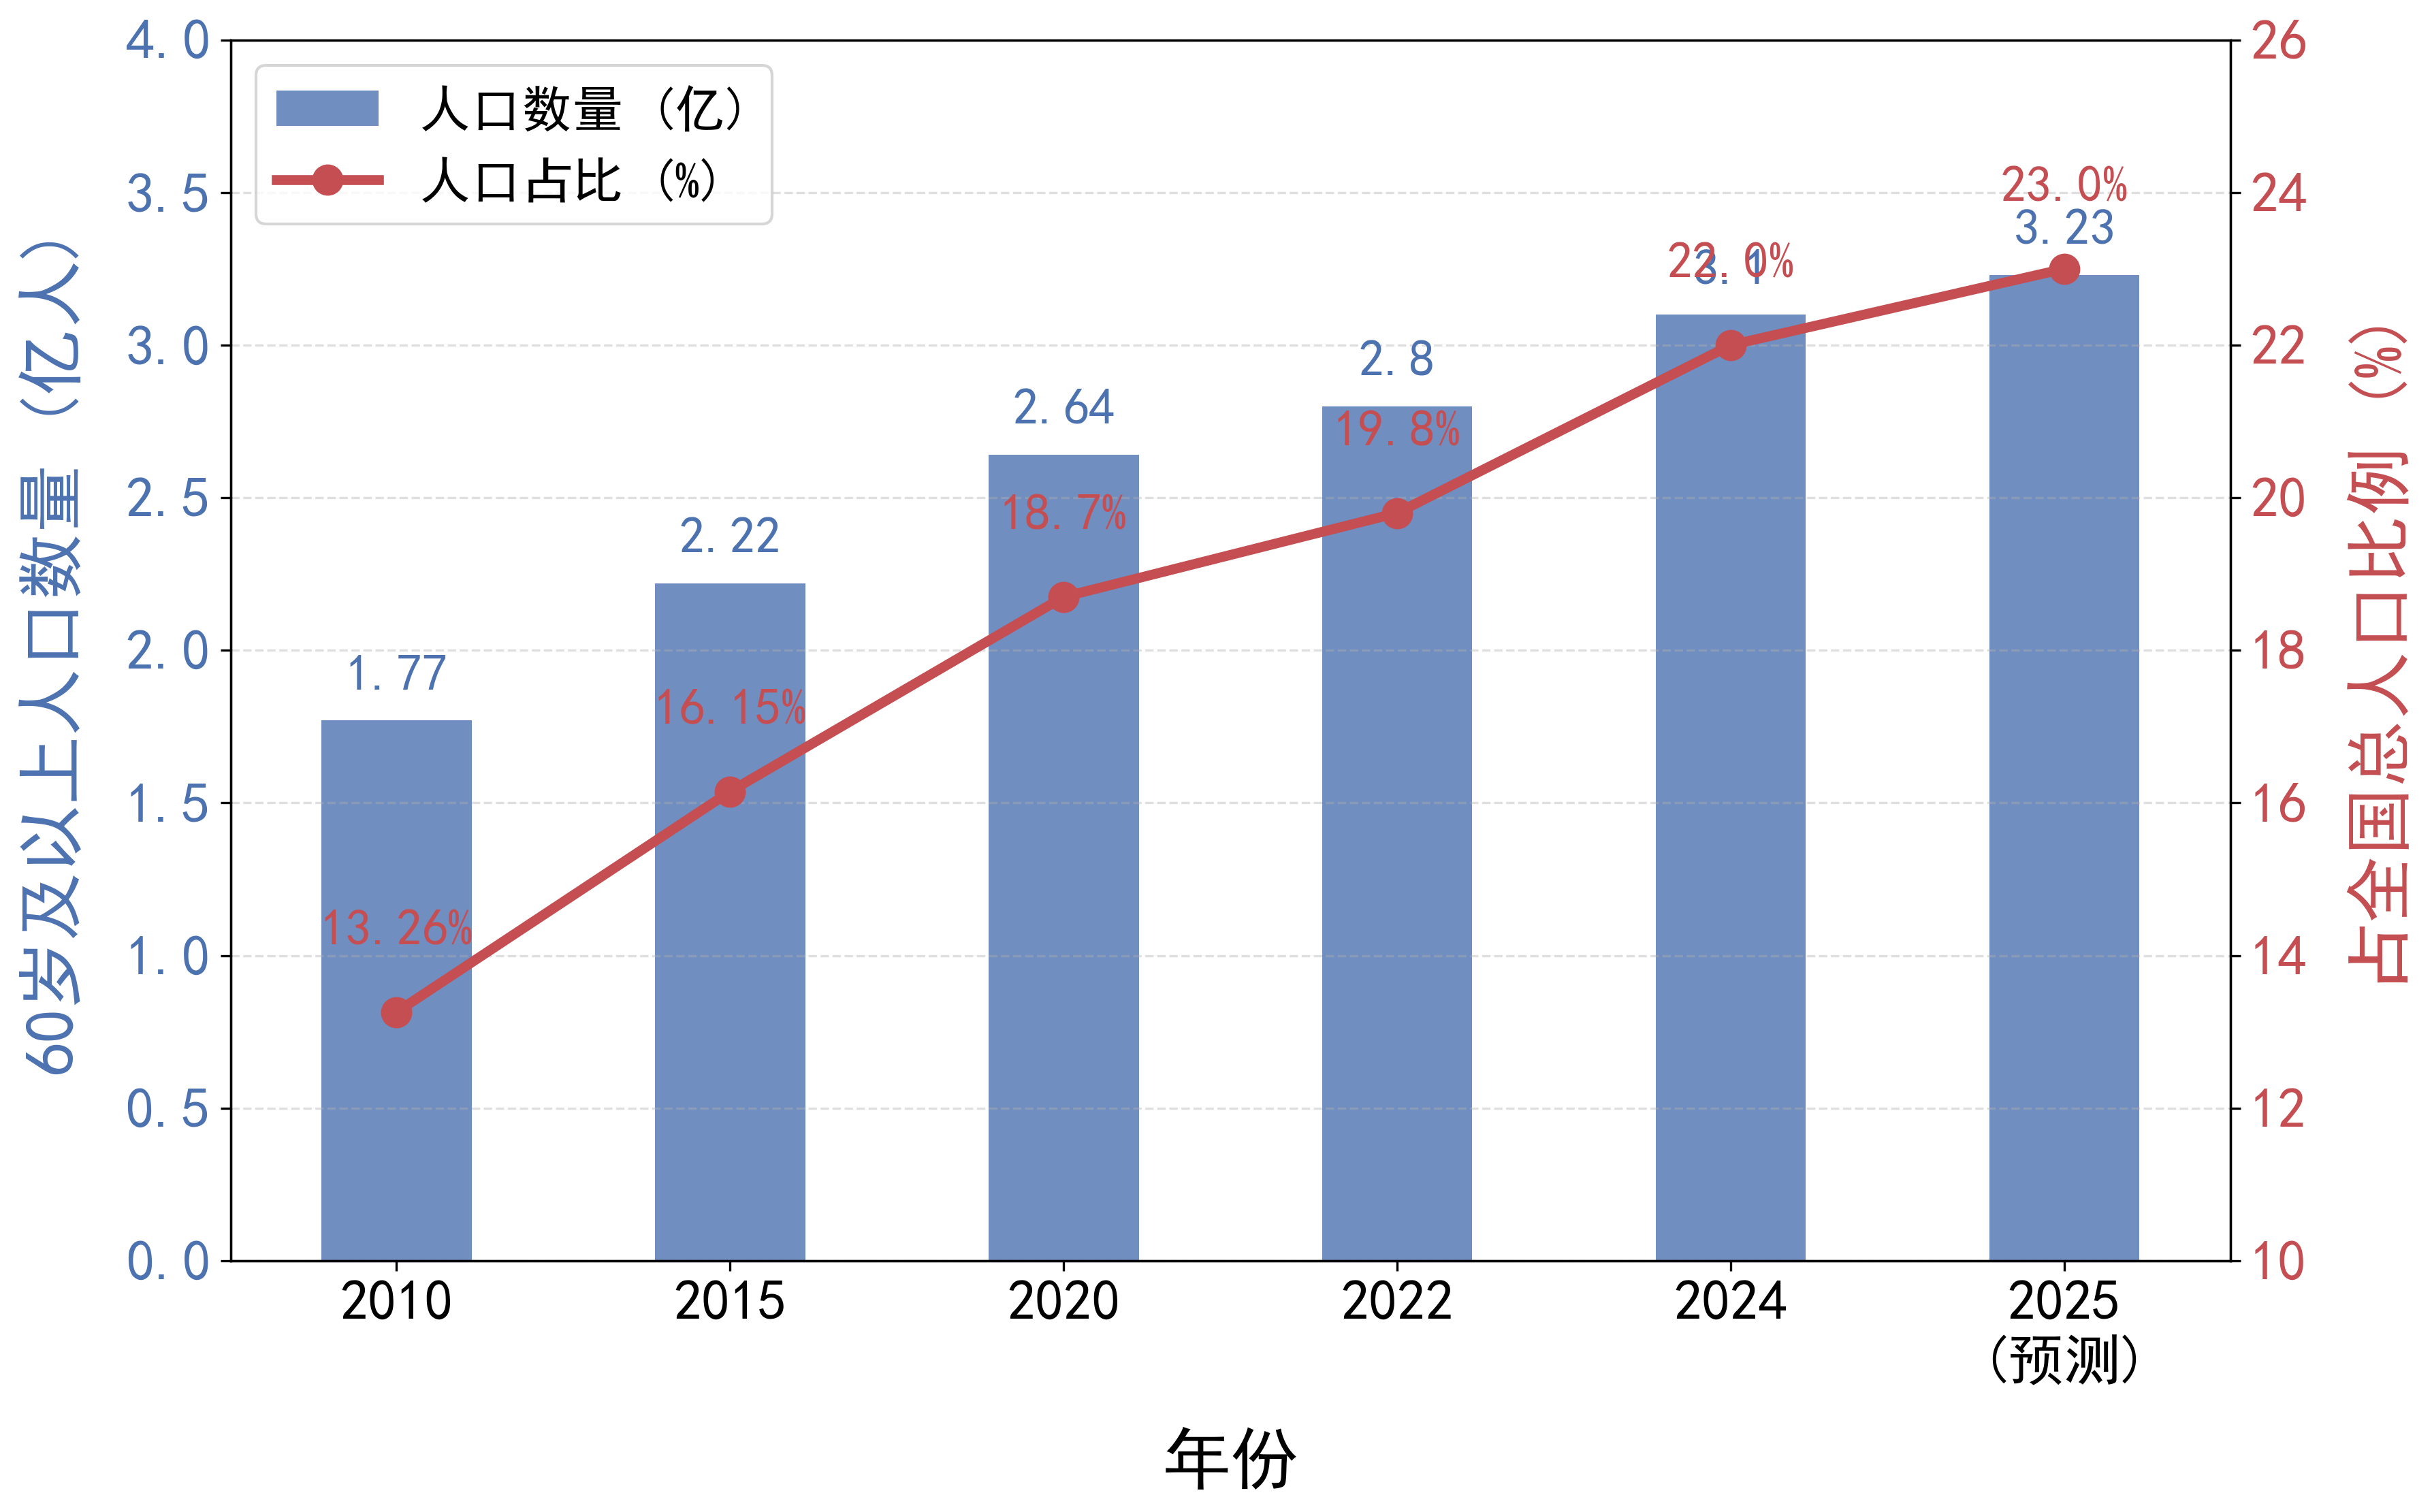
\includegraphics[width=0.85\textwidth]{figures/fig1_1_aging_population_trend.png}
    \caption{中国60岁及以上老年人口数量与占比趋势 (2010-2025)}
    \label{fig:aging_population}
\end{figure}


然而，移动终端功能的不断丰富在为大多数用户带来便利的同时，也对老年群体形成了日益突出的使用障碍。一方面，老年用户由于生理机能退化，普遍面临视力下降、听力减弱、手指灵活性降低、认知反应速度减缓等客观问题；另一方面，主流智能终端的人机交互界面设计往往以年轻用户为主要目标群体，密集的图标布局、多层嵌套的菜单结构、频繁的系统弹窗以及不断变化的应用更新，对老年人构成了显著的认知负担与操作障碍。

这种由技术快速演进与老年群体适应能力之间的差异所形成的隔阂，被学界称为“数字鸿沟”。数字鸿沟在通信领域的具体体现，包括老年人无法独立完成视频通话、容易误触系统设置导致网络中断、难以理解陌生应用界面、对授权弹窗与广告推送缺乏判断能力等。中国互联网络信息中心发布的第52次中国互联网络发展状况统计报告指出，60岁及以上网民群体占比仅为14.3\,\%\upcite{2}，远低于其在总人口中的比例，说明大量老年人在数字化浪潮中处于事实上的边缘化状态。

在通信工程专业视角下，移动通信终端不仅是数据交换的物理载体，更是承载用户与外界保持联络、获取信息、维系情感的关键媒介。如何通过终端层面的软件再设计，让老年用户重新获得对智能设备的掌控感与安全感，使其能够便捷地完成与子女的视频通话、稳定地接入家庭无线网络、流畅地使用日常应用，是当代通信工程从业者必须正视的现实命题。

\subsection{适老化痛点剖析}
从一线调研结果看，老年用户在使用主流智能手机过程中暴露出的核心痛点可归纳为以下几个方面。其一是视觉痛点，标准界面字号偏小、图标密集，导致老年人需要佩戴眼镜并凑近屏幕才能勉强辨识，长时间使用容易引发视疲劳。其二是认知痛点，多级菜单和大量弹窗使老年人难以判断当前所处的界面位置，操作过程极易迷失方向。其三是通话痛点，微信视频通话需要至少七步操作，老年人记不住流程，需要子女多次教学方能勉强掌握。其四是网络痛点，老年人误触WiFi开关后无法自行恢复连接，长时间断网而不自知，错过重要来电。其五是交互痛点，对触摸屏操作不熟练，时常出现误触或长按引发的意外操作，进一步加剧对智能设备的不安全感。

\begin{figure}[htbp]
    \centering
    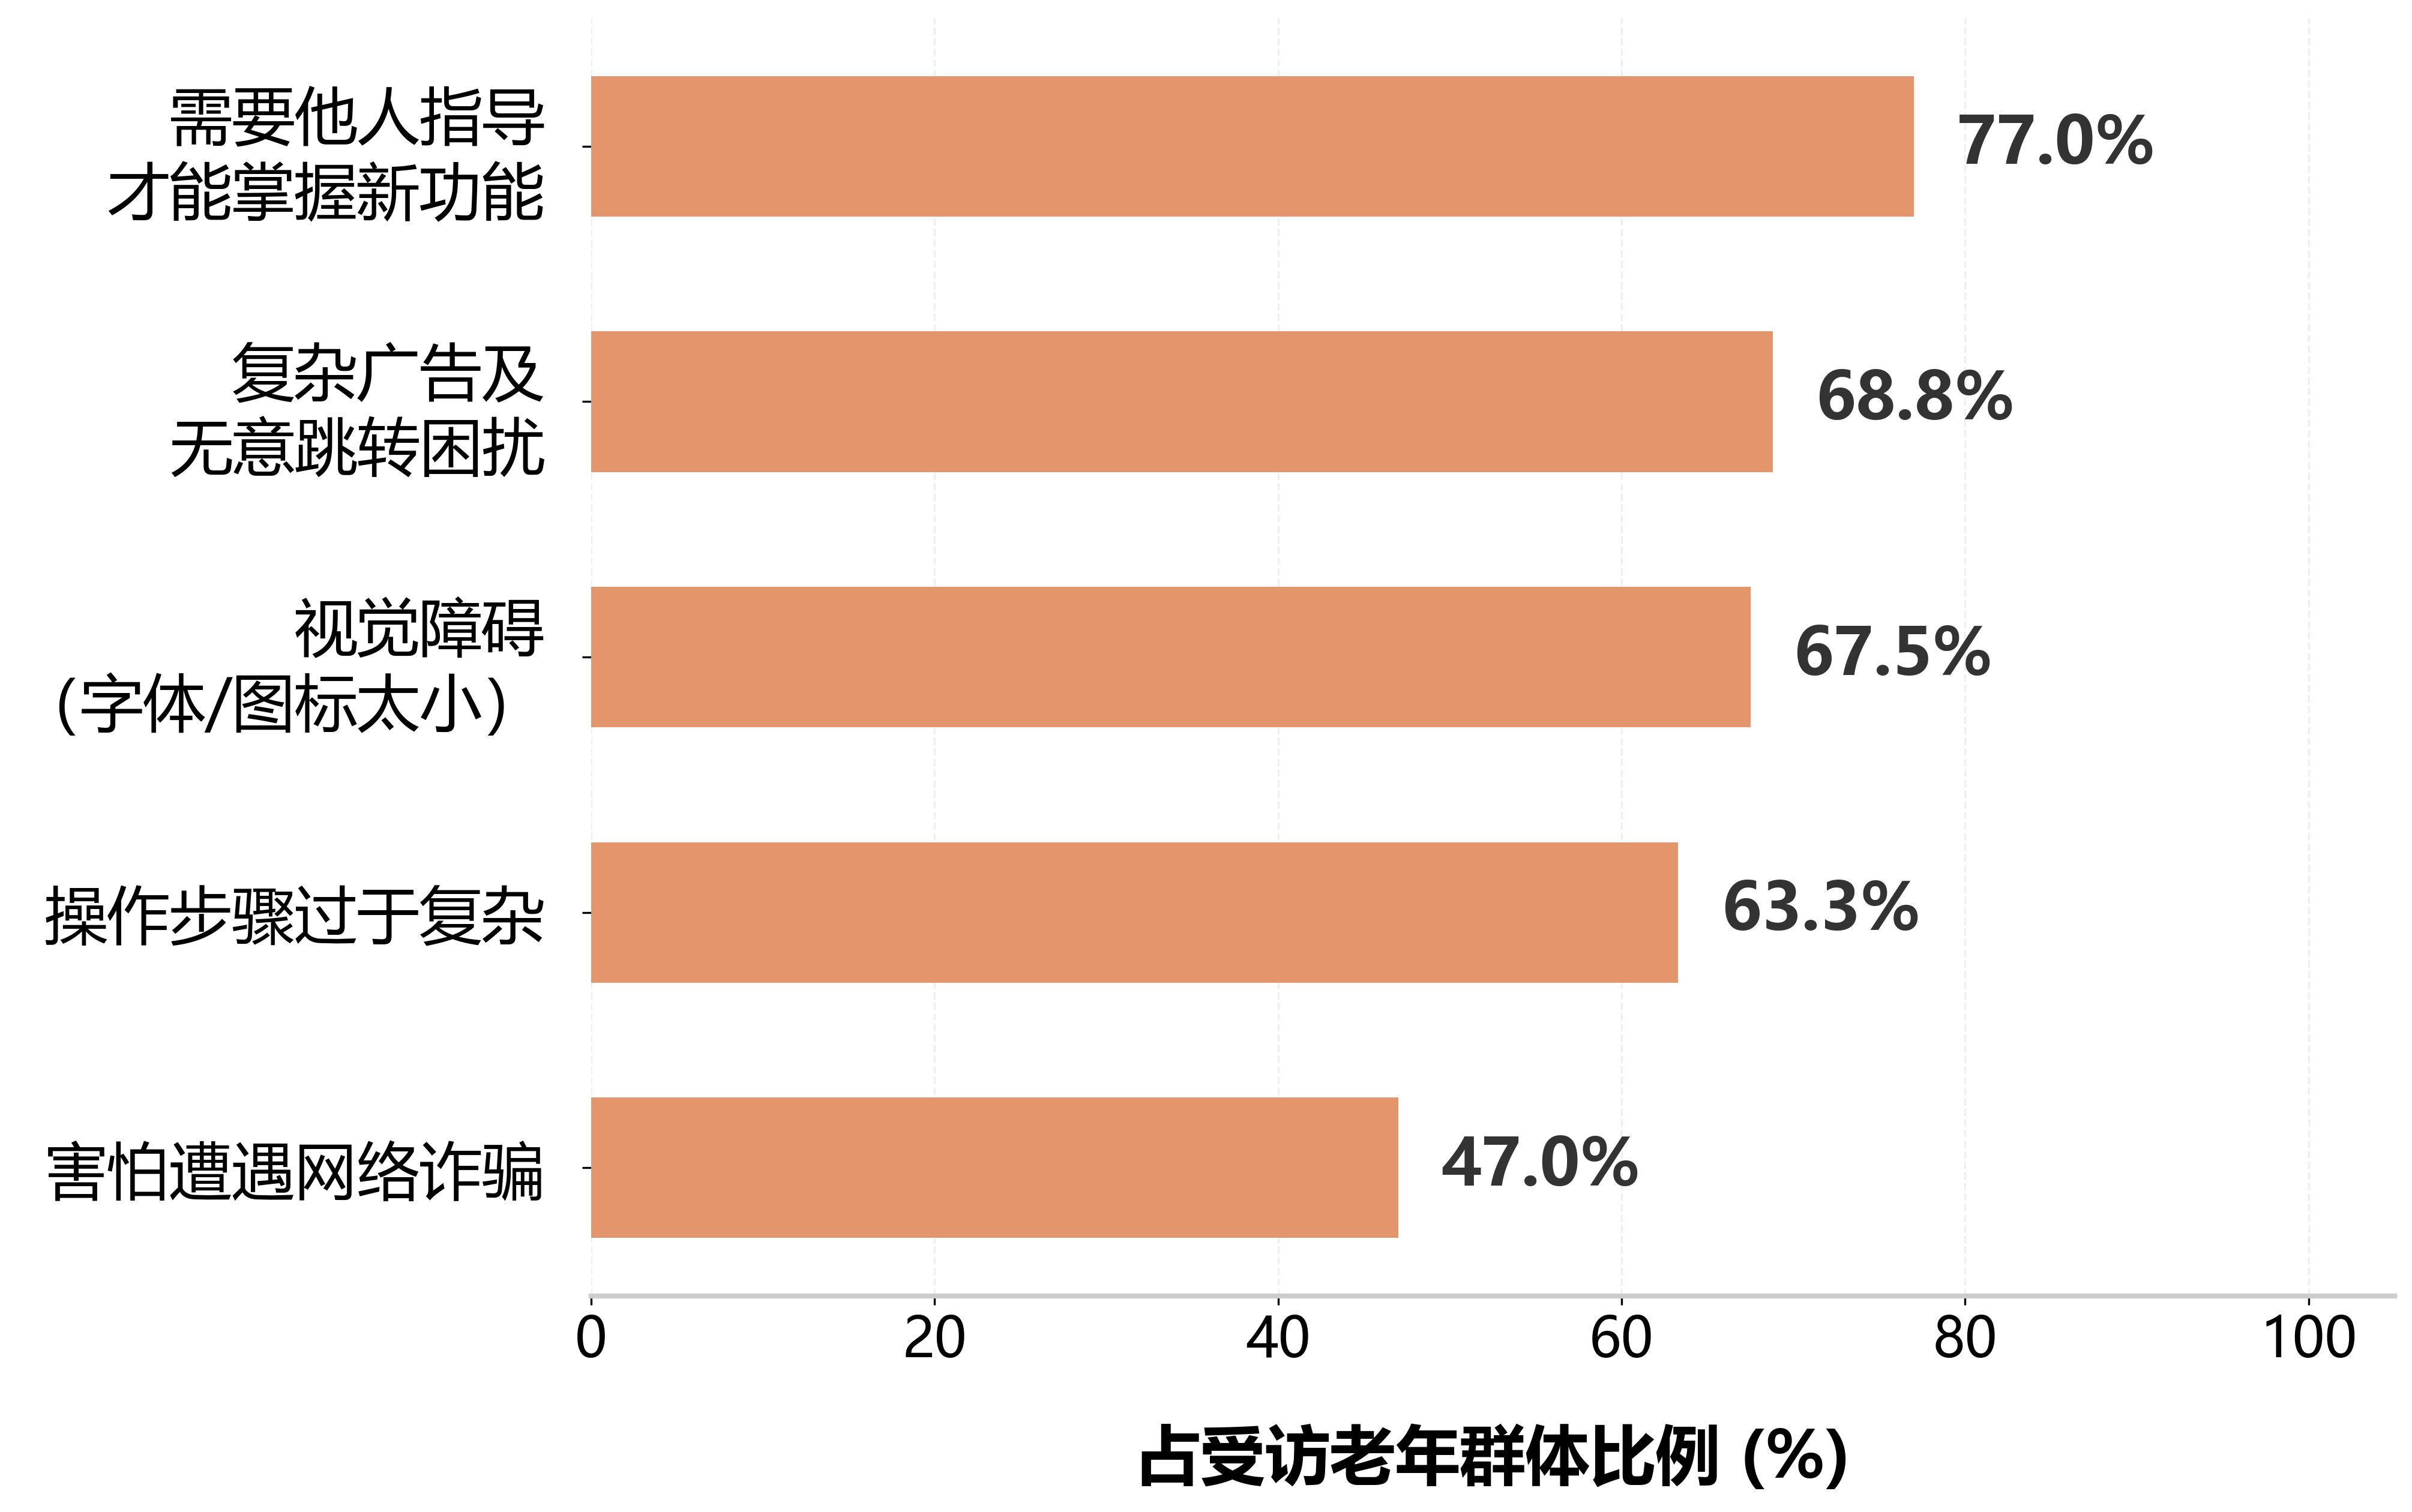
\includegraphics[width=0.85\textwidth]{figures/fig1_2_usage_pain_points.png}
    \caption{老年人智能手机使用核心痛点分布}
    \label{fig:pain_points}
\end{figure}

这些痛点的共同本质在于：现有移动通信终端的软件设计未能充分考虑老年用户的认知特征与使用习惯。仅仅通过放大字号、增大图标的浅层适老化改造，无法从根本上解决问题。必须从系统架构、交互逻辑、自动化能力等多个层面进行深度重构，才能真正为老年用户提供一款能用、好用、爱用的移动通信终端。这正是本课题立项的现实出发点。

\subsection{研究意义}
本课题以适老化智能桌面系统的设计与实现为研究对象，其意义可从社会价值、工程价值与学术价值三个维度展开。从社会价值层面看，本研究致力于通过软件技术手段帮助老年群体跨越数字鸿沟，让通信技术真正服务于全民福祉。当系统能够将原本繁琐的微信视频通话操作简化为一次点击、能够在网络异常时主动恢复并向用户清晰提示，老年用户便能更安心地依赖移动终端与家人保持联系，独居老人的精神慰藉与紧急求助通道也得到了实质性保障，这对于构建友好型老龄化社会具有积极意义。

从工程价值层面看，本课题摒弃了传统适老化方案“放大字号、堆叠图标”的简单做法，转而从系统架构与人机交互两个维度同步发力。通过自研的微内核插件化架构，系统在功能扩展性与运行稳定性方面取得了良好平衡，能够适配从千元入门机到主流旗舰机型的多种硬件配置；通过Android无障碍服务深度整合的微信一键直拨方案，系统从交互层面真正消除了老年用户的认知负担，为同类终端应用的设计提供了可复用的工程范式。

从学术价值层面看，本研究在通信终端无障碍交互、跨应用自动化控制、网络稳定性自愈等方向进行了有益探索。所提出的七阶段状态机驱动的自动化控制模型、双通道节点检索方法以及分层防御的网络守护机制，丰富了适老化通信终端研究的理论与实践成果，对推动我国老年友好型移动通信生态建设具有借鉴意义。

\section{国内外研究现状}
\subsection{移动通信终端适老化研究现状}
终端适老化是一个跨越通信工程、人机交互、工业设计等多学科的研究方向。从国际范围来看，欧美国家由于步入老龄化社会较早，相关研究起步亦较早。日本与德国的研究机构较早提出了“通用设计”理念，主张通过通用化的界面与功能设计兼顾各年龄段用户的使用需求。在产品形态上，海外市场出现了Doro、Jitterbug等专注于老年用户的终端品牌，以及Big Launcher、Simple Launcher等第三方桌面应用，其设计思路普遍以大尺寸瓷砖式布局取代传统的网格图标布局，并精简非必要功能入口。然而，海外方案在中国本土的适用性较为有限，例如其无法对国内老年用户高度依赖的微信、支付宝等应用进行深度适配，也难以兼容中国传统农历、节气等本土文化要素。

国内方面，伴随老龄化进程的加快和工信部“互联网应用适老化改造”专项行动\upcite{3}的推进，主流手机厂商相继推出了系统级适老化方案。华为的“简易模式”、小米的“极简模式”、OPPO的“简单模式”以及荣耀的“长辈模式”等，均对系统字号、图标尺寸、铃音音量等进行了适当优化，并在拦截骚扰电话、识别诈骗短信等方面提供了一定支持。但这些厂商方案的共同局限在于，其作用范围仅限于操作系统层面，无法穿透至第三方应用内部。换言之，老年用户进入微信、支付宝等具体应用后，依然需要面对其原本的复杂界面，操作障碍并未得到根本解决。

\begin{figure}[htbp]
    \centering
    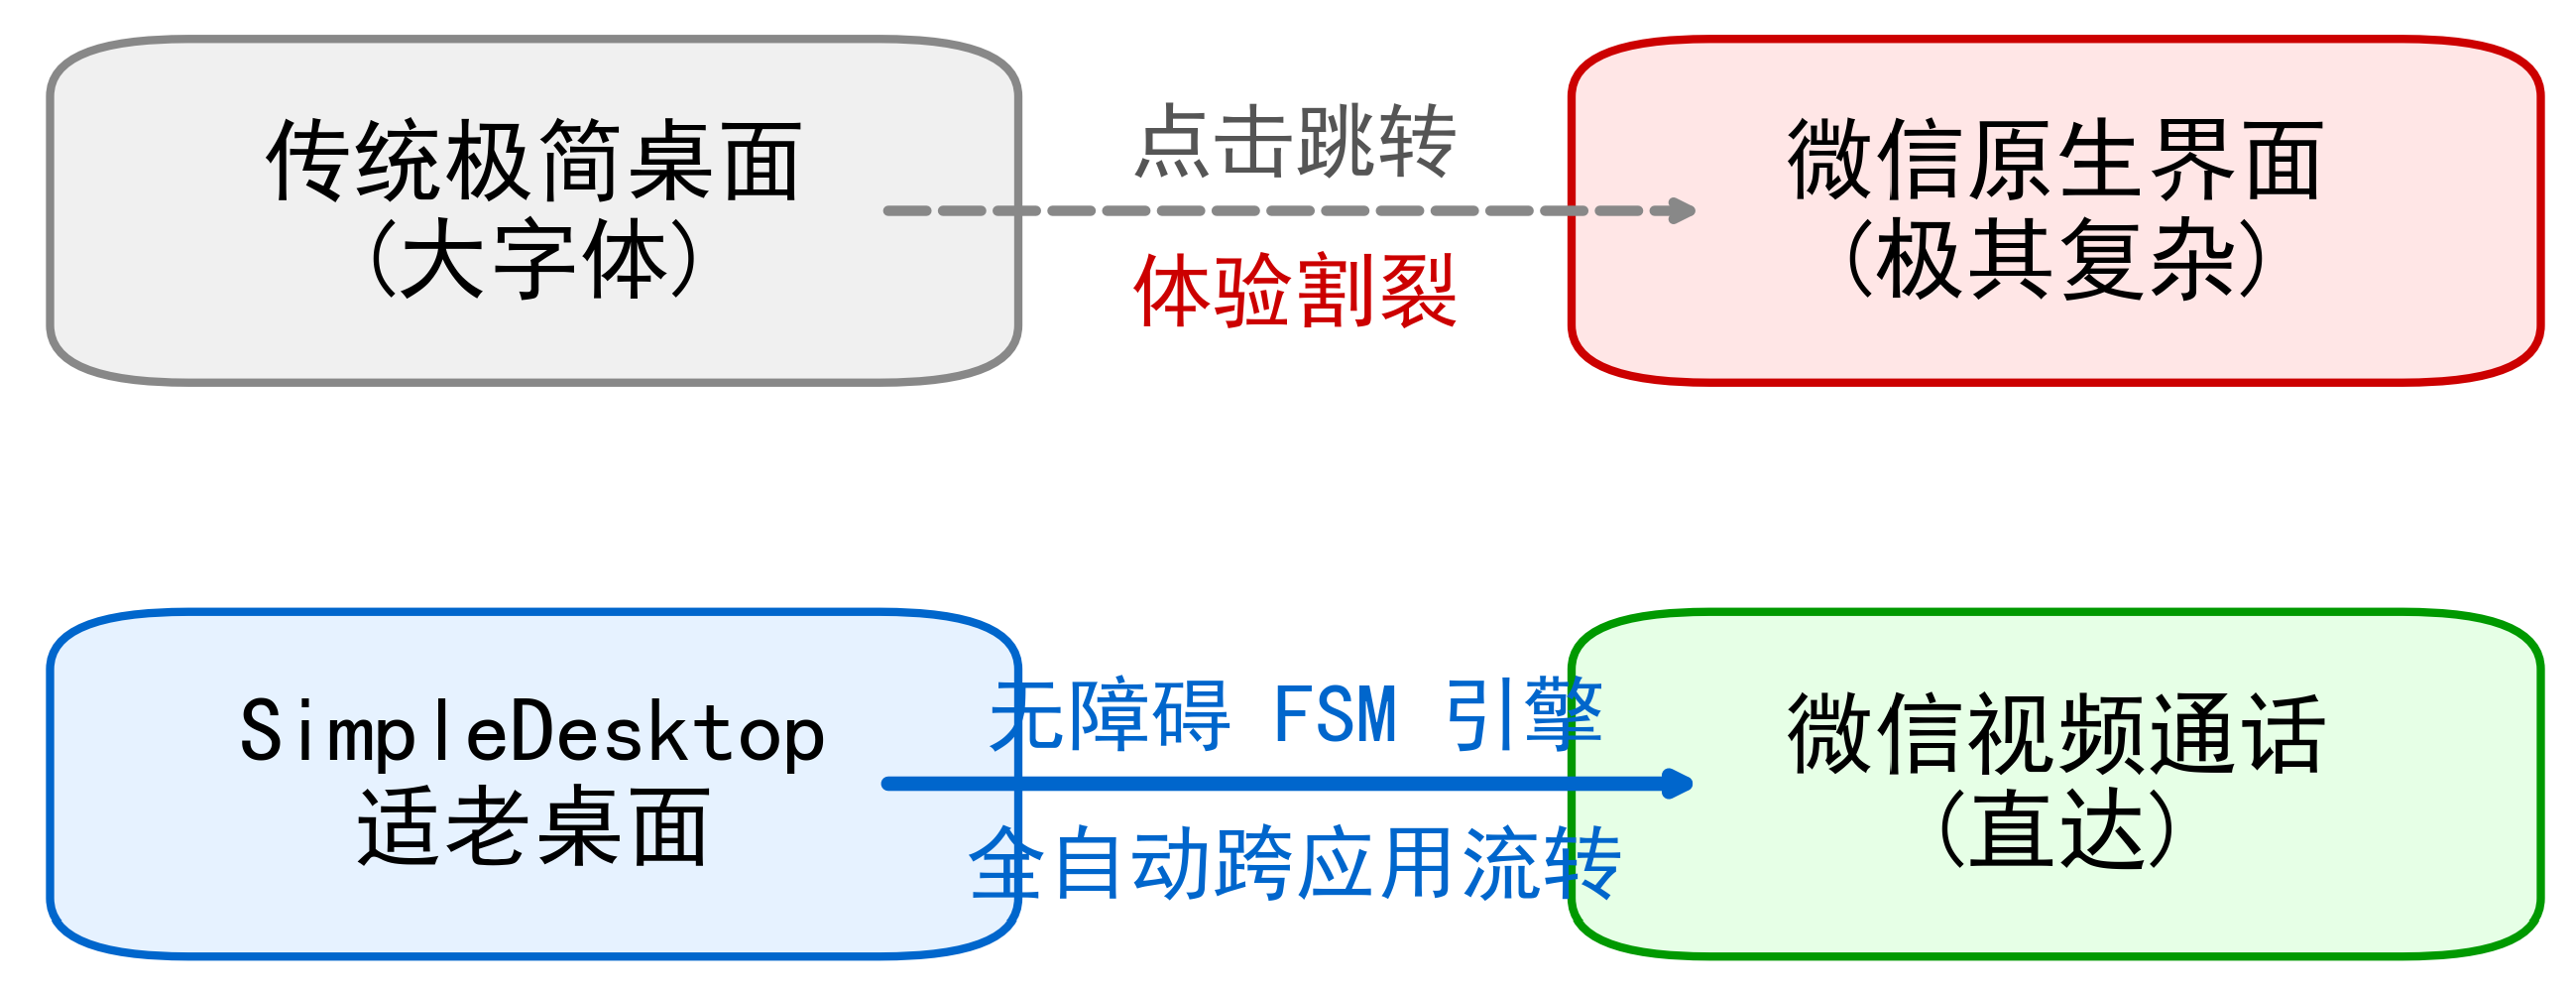
\includegraphics[width=0.9\textwidth]{figures/fig1_3_architecture_compare.png}
    \caption{传统适老化桌面与本系统自动化直达通道的体验对比}
    \label{fig:arch_compare}
\end{figure}

在学术研究方面，近年来国内外学者围绕适老化终端开展了多方面探索。文献研究普遍聚焦于以下三个方向：一是基于Fitts定律的触控目标尺寸优化，从生理人因学角度论证大按钮设计的合理性；二是基于对比敏感度模型的色彩搭配研究，提出适合老年视觉特征的高对比度配色方案；三是基于眼动追踪与可用性测试的界面布局评估，验证简化界面对老年用户操作效率的提升效果。然而，相关研究多聚焦于界面表层的视觉优化\upcite{4,5,6}，鲜有研究涉及如何让老年人在第三方应用内部也能享受到简化体验这一深层次命题\upcite{8}。

\subsection{Android无障碍自动化技术研究现状}
要实现跨第三方应用的操作简化，业界普遍采用Android平台提供的无障碍服务作为技术抓手。无障碍服务最初是为视障用户提供屏幕朗读功能而设计的系统级接口，但因其具备读取屏幕控件树和执行模拟操作的能力，近年来被广泛应用于自动抢红包、自动签到、自动化测试等多种场景。

从已有的研究与产品实践来看，基于无障碍服务的自动化控制方案主要存在以下不足：首先，绝大多数实现方式依赖目标应用控件的资源标识符进行硬编码定位，一旦目标应用版本更新或启用代码混淆，自动化流程便会迅速失效；其次，缺乏对系统级弹窗、来电中断等异常情况的容错处理机制，导致流程稳定性较差；再次，普遍缺乏对老年用户场景的针对性优化，未能将自动化能力转化为面向终端用户的简洁可靠服务。

在通信终端无障碍交互方向上，既有研究多关注屏幕朗读、语音输入等输入输出层面的辅助技术，对于如何利用无障碍能力构建稳定可靠的跨应用通信桥接这一问题，缺乏系统性的工程方案。本课题正是着眼于这一研究空白，探索通过状态机建模、双通道检索、焦点退避等机制，构建具备较高鲁棒性的适老化终端自动化通信能力。

\section{主要研究内容}
针对前述移动通信终端在适老化方向上的痛点和现有研究的不足，本课题完成了一款面向老年用户的Android智能桌面系统SimpleDesktop的全栈设计与实现。系统以问题驱动为基本思路，围绕老年用户实际遇到的视觉障碍、操作障碍、通话障碍、网络障碍和交互障碍五大问题，相应展开五个方向的研究与实践。

一是面向终端架构稳定性的微内核插件化引擎研究。系统摒弃了传统单体式应用架构，将桌面信息聚合、联系人通讯、应用启动、天气服务等业务功能解耦为相互独立的功能插件，并通过统一的插件管理器和消息总线进行协调。该架构既保证了系统在低端设备上的稳定运行，也为未来扩展健康监测、智能家居控制等模块预留了清晰接口。

二是面向老年视觉与认知特征的适老化人机交互界面研究。系统基于现代声明式UI框架构建了高对比度、大字号、卡片化的桌面界面规范，支持不同字号档位与多种主题方案的实时切换，并在主屏中以聚合面板的形式集中呈现时间、农历、天气、常用联系人和常用应用，最大限度降低老年用户的视觉搜索成本。

三是面向无障碍通信的微信一键自动通话研究。针对老年用户使用微信视频通话操作步骤过多的问题，提出基于Android无障碍服务的七阶段状态机自动化方案，配合双通道节点检索算法和焦点防冲突退避机制，实现桌面点击联系人、系统自动完成全部微信操作、直接进入视频通话的一键化流程。

四是面向终端通信连续性的WiFi网络守护研究。系统通过常驻前台服务持续监测网络连接状态，一旦检测到WiFi断连便进入宽限期等待自动恢复；超过宽限期后，借助无障碍服务自动开启WiFi开关，并通过弹窗与语音播报双重通道引导用户进行必要的人工干预，从而最大限度保障通信链路的连续性。

五是面向自然语言交互的语音助手研究。系统基于Android原生TTS引擎实现全局语音播报，并通过关键词匹配与编辑距离容错相结合的轻量级语义解析方法，将打电话给某某等自然语言指令准确映射到具体的通信操作上，使老年用户无需依赖屏幕触控即可完成主要操作。

\begin{figure}[htbp]
    \centering
    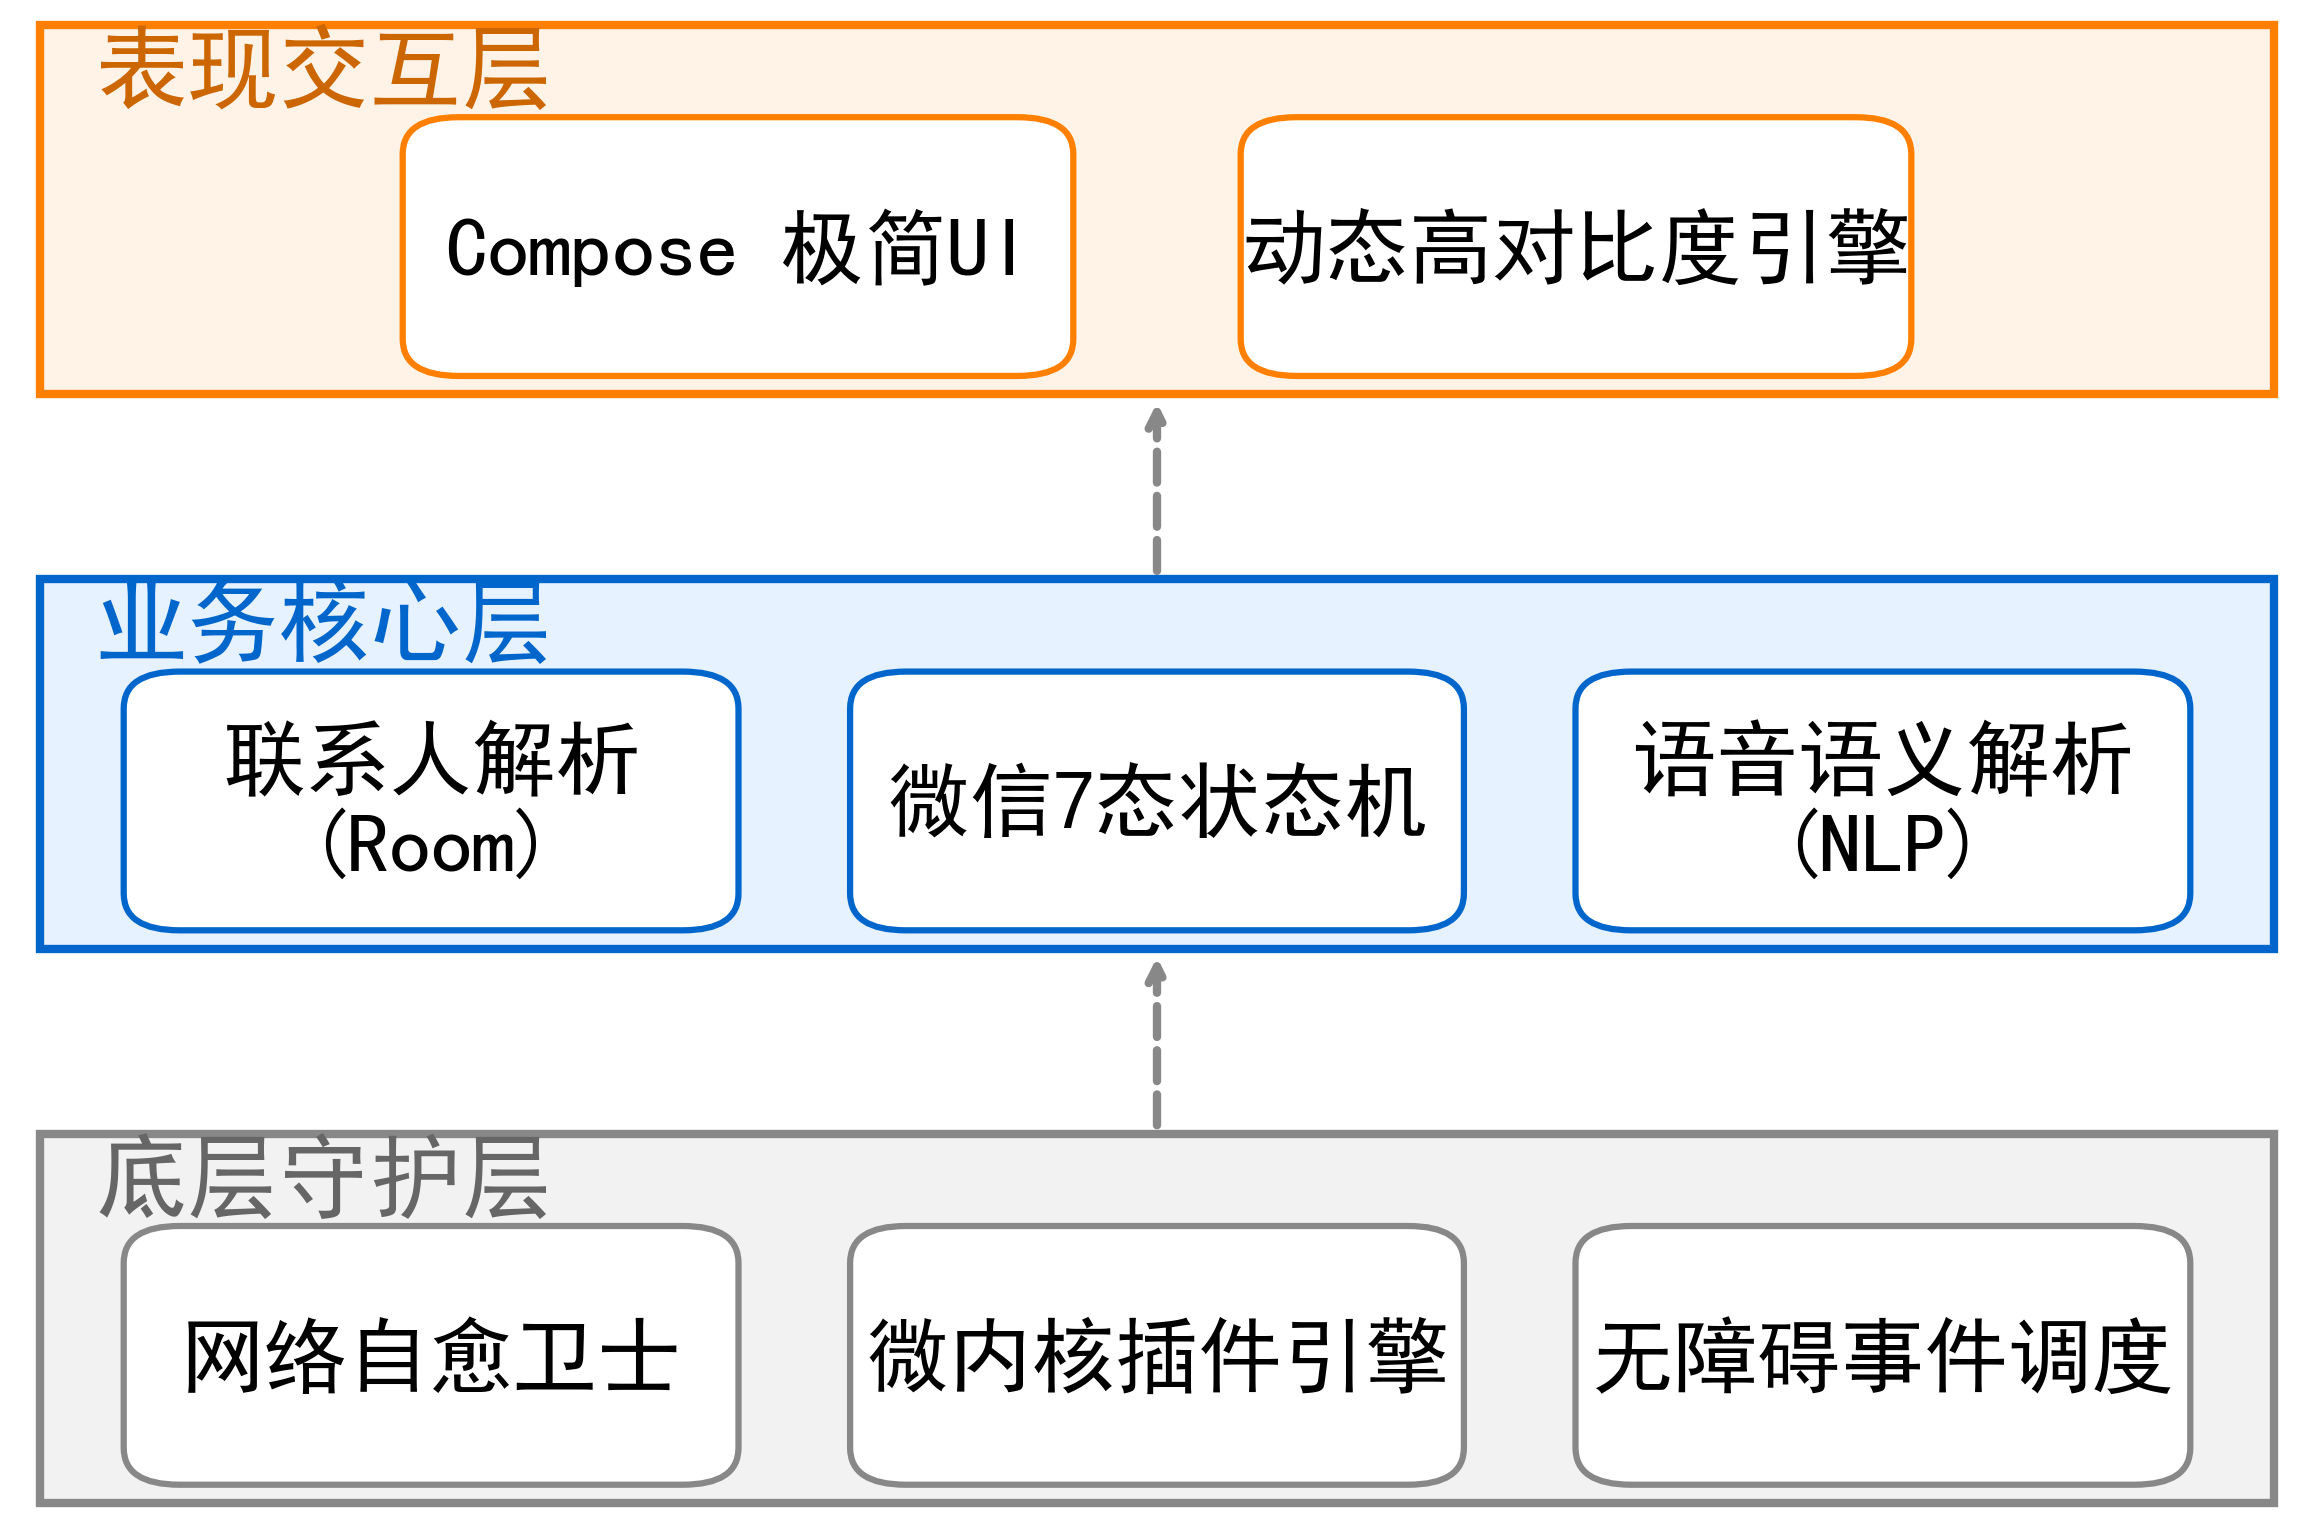
\includegraphics[width=0.9\textwidth]{figures/fig1_4_system_overview.png}
    \caption{SimpleDesktop 系统技术全景架构图}
    \label{fig:system_overview}
\end{figure}

\section{论文组织结构}
全文共分五章，各章主要内容如下。

第1章为绪论，主要介绍课题的研究背景、研究意义、国内外研究现状、主要研究内容以及论文的组织结构，旨在明确研究的出发点与全文的整体脉络。

第2章为技术基础，主要介绍本课题所依赖的技术体系，包括现代Android技术栈、数据持久化与依赖注入框架、微内核插件化架构理论以及Android无障碍服务的基本原理，为后续章节的设计与实现奠定理论与技术基础。

第3章为适老化智能桌面系统的设计与实现，是论文的核心章节。首先从老年用户视角出发开展需求分析，然后给出宿主层、总线层、插件层三层架构的整体设计方案并交代开发环境，接着分别对适老化界面、微信自动化直连、WiFi网络守护、语音辅助等核心功能模块进行设计与实现的详细阐述，最后给出软件的整体操作流程。

第4章为软件测试与分析，依次从功能测试、兼容性测试和性能测试三个维度对系统质量进行系统化评估。功能测试覆盖联系人增删改查、应用管理、微信通话发起、语音指令解析等核心用例；兼容性测试覆盖不同型号、不同分辨率、不同系统版本的真机环境；性能测试关注响应时间、页面加载速度以及多并发访问的处理能力。

第5章为总结与展望。首先对全文工作进行总结，凝练课题的主要成果与贡献；其次客观分析当前系统存在的局限性，并对未来的研究方向作出展望。


\begin{table}
    \small
    \caption{表格内换行文字单倍行距测试}
    \label{tab:linebreak_test}
    \begin{threeparttable}
    \begin{tabular}{c p{4cm} p{4cm}}
        \toprule
        \tableheader{编号} & \tableheader{描述} & \tableheader{详细说明} \\
        \midrule
        \tablecell{001} & \tablecell{基础测试项目} & \tablecell{这是一个包含多行文字的测试内容，用于验证表格内换行文字的单倍行距效果是否正确实现。} \\
        \tablecell{002} & \tablecell{高级功能验证} & \tablecell{第二行测试内容，包含较长的文字描述，需要自动换行显示，确保行间距为单倍行距设置。} \\
        \tablecell{003} & \tablecell{综合评估测试*} & \tablecell{第三个测试项目，用于验证表格脚注与换行文字的配合效果，确保所有格式要求都得到满足。} \\
         \bottomrule
    \end{tabular}
    \begin{tablenotes}
        \songti\fontsize{11pt}{11pt}\selectfont
        \item[*] 这是一个带有脚注的测试项目，用于验证表格脚注格式与单倍行距的配合效果。
    \end{tablenotes}
    \end{threeparttable}
\end{table}


% \iffalse



fig1_1_aging_population_trend.pdf / .png
内容：中国60岁及以上老年人口数量与占比趋势图（2010-2025年）。
用途：基于国家统计局数据，包含柱状图与折线图的双轴设计，呈现学术蓝与红的配色，极其适合放在 1.1.1 时代背景 中。
fig1_2_usage_pain_points.pdf / .png
内容：老年人智能手机使用核心痛点分布条形图。
用途：基于 CNNIC 等调研机构数据，直观展示了由于弹窗广告、操作繁琐导致的痛点比例，适合放在数字鸿沟论述的末尾。




\begin{table}
    \small
    \caption{表格内换行文字单倍行距测试}
    \label{tab:linebreak_test}
    \begin{threeparttable}
    \begin{tabular}{c p{4cm} p{4cm}}
        \toprule
        \tableheader{编号} & \tableheader{描述} & \tableheader{详细说明} \\
        \midrule
        \tablecell{001} & \tablecell{基础测试项目} & \tablecell{这是一个包含多行文字的测试内容，用于验证表格内换行文字的单倍行距效果是否正确实现。} \\
        \tablecell{002} & \tablecell{高级功能验证} & \tablecell{第二行测试内容，包含较长的文字描述，需要自动换行显示，确保行间距为单倍行距设置。} \\
        \tablecell{003} & \tablecell{综合评估测试*} & \tablecell{第三个测试项目，用于验证表格脚注与换行文字的配合效果，确保所有格式要求都得到满足。} \\
         \bottomrule
    \end{tabular}
    \begin{tablenotes}
        \songti\fontsize{11pt}{11pt}\selectfont
        \item[*] 这是一个带有脚注的测试项目，用于验证表格脚注格式与单倍行距的配合效果。
    \end{tablenotes}
    \end{threeparttable}
\end{table}

第一章内容，这里是第二节的第二小节的内容。第一章内容，这里是第二节的第二小节的内容。第一章内容，这里是第二节的第二小节的内容。第一章内容，这里是第二节的第二小节的内容。第一章内容，这里是第二节的第二小节的内容。根据经典著作，深度学习的基础理论已经相当完善。
第一章内容，这里是第二节的第二小节的内容。第一章内容，这里是第二节的第二小节的内容。第一章内容，这里是第二节的第二小节的内容。第一章内容，这里是第二节的第二小节的内容。第一章内容，这里是第二节的第二小节的内容。第一章内容，这里是第二节的第二小节的内容。
第一章内容，这里是第二节的第二小节的内容。第一章内容，这里是第二节的第二小节的内容。第一章内容，这里是第二节的第二小节的内容。第一章内容，这里是第二节的第二小节的内容。第一章内容，这里是第二节的第二小节的内容。第一章内容，这里是第二节的第二小节的内容。
第一章内容，这里是第二节的第二小节的内容。第一章内容，这里是第二节的第二小节的内容。第一章内容，这里是第二节的第二小节的内容。第一章内容，这里是第二节的第二小节的内容。第一章内容，这里是第二节的第二小节的内容。第一章内容，这里是第二节的第二小节的内容。
第一章内容，这里是第二节的第二小节的内容。第一章内容，这里是第二节的第二小节的内容。第一章内容，这里是第二节的第二小节的内容。第一章内容，这里是第二节的第二小节的内容。第一章内容，这里是第二节的第二小节的内容。第一章内容，这里是第二节的第二小节的内容。
第一章内容，这里是第二节的第二小节的内容。第一章内容，这里是第二节的第二小节的内容。第一章内容，这里是第二节的第二小节的内容。第一章内容，这里是第二节的第二小节的内容。第一章内容，这里是第二节的第二小节的内容。第一章内容，这里是第二节的第二小节的内容。
第一章内容，这里是第二节的第二小节的内容。第一章内容，这里是第二节的第二小节的内容。第一章内容，这里是第二节的第二小节的内容。第一章内容，这里是第二节的第二小节的内容。第一章内容，这里是第二节的第二小节的内容。第一章内容，这里是第二节的第二小节的内容。

\begin{figure}[h]
    \centering
    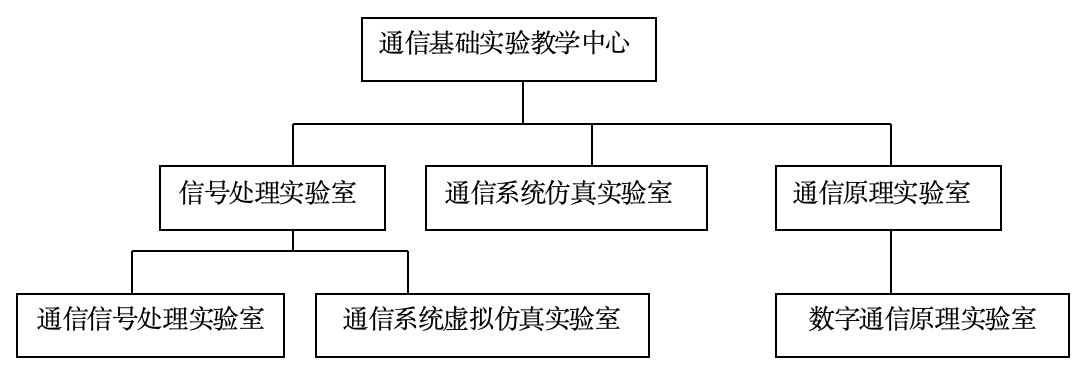
\includegraphics[width=0.8\textwidth]{figures/pic.png}
    \caption{这是一张图片的说明(图中的字体是图片生成的时候设置的，这里是宋体 11pt)}
    \label{fig:example}
\end{figure}

第一章内容，这里是第二节的第二小节的内容。第一章内容，这里是第二节的第二小节的内容。第一章内容，这里是第二节的第二小节的内容。第一章内容，这里是第二节的第二小节的内容。第一章内容，这里是第二节的第二小节的内容。第一章内容，这里是第二节的第二小节的内容。
第一章内容，这里是第二节的第二小节的内容。第一章内容，这里是第二节的第二小节的内容。第一章内容，这里是第二节的第二小节的内容。第一章内容，这里是第二节的第二小节的内容。第一章内容，这里是第二节的第二小节的内容。第一章内容，这里是第二节的第二小节的内容。
第一章内容，这里是第二节的第二小节的内容。第一章内容，这里是第二节的第二小节的内容。第一章内容，这里是第二节的第二小节的内容。第一章内容，这里是第二节的第二小节的内容。第一章内容，这里是第二节的第二小节的内容。第一章内容，这里是第二节的第二小节的内容。
第一章内容，这里是第二节的第二小节的内容。第一章内容，这里是第二节的第二小节的内容。第一章内容，这里是第二节的第二小节的内容。第一章内容，这里是第二节的第二小节的内容。第一章内容，这里是第二节的第二小节的内容。第一章内容，这里是第二节的第二小节的内容。
第一章内容，这里是第二节的第二小节的内容。第一章内容，这里是第二节的第二小节的内容。第一章内容，这里是第二节的第二小节的内容。第一章内容，这里是第二节的第二小节的内容。第一章内容，这里是第二节的第二小节的内容。第一章内容，这里是第二节的第二小节的内容。
第一章内容，这里是第二节的第二小节的内容。第一章内容，这里是第二节的第二小节的内容。第一章内容，这里是第二节的第二小节的内容。第一章内容，这里是第二节的第二小节的内容。第一章内容，这里是第二节的第二小节的内容。第一章内容，这里是第二节的第二小节的内容。
第一章内容，这里是第二节的第二小节的内容。第一章内容，这里是第二节的第二小节的内容。第一章内容，这里是第二节的第二小节的内容。第一章内容，这里是第二节的第二小节的内容。第一章内容，这里是第二节的第二小节的内容。第一章内容，这里是第二节的第二小节的内容。

\fi